%=========================================================================
% (c) Michal Bidlo, Bohuslav Křena, 2008

% tikzit regex: (,)?\s*style=\w*(,)?\s*

% \listoftodos

\chapter{Introduction}
Nowadays, when malicious code or malware is becoming more and more sophisticated and pressing security risk, it is really needed to control a program behavior and monitor what the program is doing in a system.
Monitoring program behavior can be done in many ways and one of the easiest ways is to use Intrusion Detection System (IDS).
IDS is an out-of-the-box solution which can monitor i.e. where program wrote or read something, and it is not allowed.
After that, IDS is reporting this violation.

Another way is to monitor and block system calls (syscalls).
Monitoring is performed using tools mentioned in the next chapter.
The actual blocking can be performed with mandatory access control (MAC) (Apparmor, SELinux), sandboxing (seccomp) or others mechanisms.
MAC refers to a type of access control by which the operating system constraints the ability of a subject or initiator to access or generally perform some sort of operation on an object or target.
Seccomp is a Linux kernel module which allows a process one-way transition to secure a state where the process can only use four syscalls.
When the process tries to call another syscall then one of the four member's sets is terminated with SIGKILL.
The set of allowed system calls can be extended using seccomp-bpf.
This extension allows filtering system calls using a configurable policy implemented with Berkley Packet Filter (BPF) rules.
This last part is an area on which I would like to focus in my thesis.

I aim to design and develop a tool which helps developers using libseccomp and seccomp-bpf.
I plan to create policies for a specific program in a format readable by libseccomp or seccomp-bpf.

\Cref{chap:syscalls} describes syscalls and how to monitor them.
In the chapter \Cref{chap:third} of the thesis, I will illustrate how security facilities in Linux, such as systrace and seccomp, work.
After the theoretical part, the design and development of a tool will follow.
In conclusion, methodology how this tool was tested is described.

\chapter{System Calls and Monitoring Tools}
\label{chap:syscalls}
In this chapter, I will describe the term system call and make an overview of tools which can monitor the system calls.
We will focus in detail on the strace tool which will be used as an input to my tool.
The other applications are described briefly not as detailed as the strace tool.

\section{System Calls}

In computer terminology, the term syscall is a way in which a computer program requests a service of the operating system on which is executed on.
In other words, system calls are functions used in the kernel itself.
The system call appears to a standard developer as a C function call.
This design is typical for monolithic kernels.
We can find them on every UNIX system.
The system call can be called on Linux/i86 multiple ways. One of them is to call interruption no. \texttt{0x80} with value of syscall in register \texttt{eax}.
The second and third one is by calling system calls \texttt{syscall()} or \texttt{sysenter()} and these syscalls are handled by the kernel in a privileged mode.
When a user invokes a system call, an execution flow is as follows:
\begin{itemize}
	\item Each syscall is vectored through a stub in libc.
    	  Some syscalls are more complicated than others because of a variable length of the arguments, but the entry point and the end point of syscall are still the same.
	\item In libc, the number of the syscall is then set to an \texttt{eax} register, and the stack frame is also set up.
	\item An interrupt number \texttt{0x80} is called and transferred to the kernel entry point.
    	  The entry point is the same for every system call.
	\item In the table of interrupts, a pointer to interruption handler is found.
    	  After that, the execution of the interrupt handler follows which stores the content of the CPU registers and checks if a valid syscall is called.
	\item The handler finds the corresponding offset in the table of interrupts \texttt{\_sys\_call\_table}, where a pointer to the syscall service is stored.
	\item Control is transferred to the syscall service.
	\item Syscall returns a value to the register \texttt{EAX} on a 32-bit architecture or \texttt{RAX} on a 64-bit architecture.
	\item At the end of the syscall, \texttt{\_ret\_from\_sys\_call\(\)} is called.
    	  This call is done before returning to user space.
          It checks if the scheduler should be run, and if so, it calls it.
	\item Immediately after return from the system call to interrupt handler, \texttt{syscallX()} macro checks for a negative return value from the syscall, if so it puts a positive copy of a return value to a global variable \texttt{\_errno}, for accessing from code like \texttt{perror()}.
\end{itemize}

This procedure is illustrated in Figure \ref{fig:tikz:int_handling}. \cite{Silberschatz2013}

\begin{figure}[]
  \centering
  % \includestandalone[]{obrazky-figures/mytikz}%     without .tex extension
  \begin{tikzpicture}[align=left, thick]
	\begin{pgfonlayer}{nodelayer}
		\node [] (0) at (-5, 5) {};
		\node [] (1) at (-4, 5) {};
		\node [] (2) at (-5, 3.75) {};
		\node [] (3) at (-4, 3.75) {};
		\node [] (4) at (-2, 6) {};
		\node [] (5) at (-2, 3.25) {};
		\node [] (6) at (1, 3.25) {};
		\node [] (7) at (1, 6) {};
		\node [] (8) at (-4, 4.5) {};
		\node [] (9) at (-4, 4.25) {};
		\node [] (10) at (-2, 4.5) {};
		\node [] (11) at (-2, 4.25) {};
		\node [] (12) at (-5, 4.5) {};
		\node [] (13) at (-6, 4.5) {};
		\node [] (14) at (-6, 2) {};
		\node [] (15) at (-8, 2) {};
		\node [] (16) at (2.25, 2) {};
		\node [] (17) at (-6, 1) {};
		\node [] (18) at (-8, 1) {};
		\node [] (19) at (-6.25, 1) {};
		\node [] (20) at (-5.75, 1) {};
		\node [] (21) at (-4.25, 1) {};
		\node [] (22) at (-4.25, -0) {};
		\node [] (23) at (-5.75, -0) {};
		\node [] (24) at (-6, -0) {};
		\node [] (25) at (-6.25, -0) {};
		\node [] (26) at (-8, -0) {};
		\node [] (27) at (-6, 0.5) {};
		\node [] (28) at (-4.5, -0.75) {};
		\node [] (29) at (-4.5, -1.75) {};
		\node [] (30) at (-3.5, -1.75) {};
		\node [] (31) at (-3.5, -0.75) {};
		\node [] (32) at (-4, -1.25) {};
		\node [] (33) at (-4.5, -1.25) {};
		\node [] (34) at (-2, -0) {};
		\node [] (35) at (-2, -2.5) {};
		\node [] (36) at (-1, -2.5) {};
		\node [] (37) at (-1, -0) {};
		\node [] (38) at (-2, -0.75) {};
		\node [] (39) at (-1, -0.75) {};
		\node [] (40) at (-1, -1.25) {};
		\node [] (41) at (-2, -1.25) {};
		\node [] (42) at (0, -0) {};
		\node [] (43) at (1, -0) {};
		\node [] (44) at (1, -1) {};
		\node [] (45) at (0, -1) {};
		\node [] (46) at (0, -1.75) {};
		\node [] (47) at (1, -1.75) {};
		\node [] (48) at (1, -2.75) {};
		\node [] (49) at (0, -2.75) {};
		\node [] (50) at (-1.5, -1) {};
		\node [] (51) at (0, -0.5) {};
		\node [] (52) at (-2, -1) {};
		\node [] (53) at (-3.75, -0.5) {};
		\node [] (54) at (0.5, -0) {};
		\node [] (55) at (-4, -0.5) {};
		\node [] (56) at (-4.25, 3.5) {};
		\node [font={\tiny}, right, align=left,] (57) at (-7.75, 2.25) {User space};
		\node [font={\tiny}, right, align=left,] (58) at (-7.75, 1.75) {Kernel space};
		\node [align=left, rotate=270, font=\small] (59) at (-5.75, 3) {\texttt{int \$0x80}};
		\node [] (60) at (-4.5, 5.25) {libc};
		\node [] (61) at (-0.5, 6.25) {source.c};
		\node [font={\small}, align=left,] (62) at (-0.75, 5.5) {int main()\{};
		\node [font={\small}, align=left,] (63) at (-0.25, 5) {printf("42")\;};
		\node [font={\small}, align=left,] (64) at (-0.5, 4.5) {return 0;};
		\node [font={\small}, align=left,] (65) at (-1.5, 4) {\}};
		\node [] (66) at (-4, -2.25) {};
	\end{pgfonlayer}
	\begin{pgfonlayer}{edgelayer}
		\draw [] (0.center) to (1.center);
		\draw [] (0.center) to (2.center);
		\draw [] (2.center) to (3.center);
		\draw [] (3.center) to (9.center);
		\draw [] (9.center) to (8.center);
		\draw [] (8.center) to (1.center);
		\draw [->, thick] (8.center) to (10.center);
		\draw [<-, loosely dashed, thick, in=180, out=0, looseness=1.00] (9.center) to (11.center);
		\draw [] (11.center) to (10.center);
		\draw [] (4.center) to (10.center);
		\draw [] (5.center) to (11.center);
		\draw [] (5.center) to (6.center);
		\draw [] (6.center) to (7.center);
		\draw [] (7.center) to (4.center);
		\draw [thick,] (12.center) to (13.center);
		\draw [thick,] (13.center) to (14.center);
		\draw [ultra thick,] (14.center) to (15.center);
		\draw [, ultra thick] (14.center) to (16.center);
		\draw [thick, ->] (14.center) to (17.center);
		\draw [] (17.center) to (20.center);
		\draw [] (20.center) to (21.center);
		\draw [] (22.center) to (23.center);
		\draw [] (20.center) to (23.center);
		\draw [] (23.center) to (24.center);
		\draw [] (24.center) to (25.center);
		\draw [] (25.center) to (19.center);
		\draw [] (19.center) to (17.center);
		\draw [] (19.center) to (18.center);
		\draw [] (18.center) to (26.center);
		\draw [] (26.center) to (25.center);
		\draw [] (28.center) to (33.center);
		\draw [] (33.center) to (29.center);
		\draw [] (29.center) to (30.center);
		\draw [] (31.center) to (28.center);
		\draw [thick, ->, in=180, out=-90, looseness=1.25] (27.center) to (33.center);
		\draw [] (38.center) to (41.center);
		\draw [] (41.center) to (40.center);
		\draw [] (40.center) to (39.center);
		\draw [] (39.center) to (38.center);
		\draw [] (38.center) to (34.center);
		\draw [] (34.center) to (37.center);
		\draw [] (37.center) to (39.center);
		\draw [] (40.center) to (36.center);
		\draw [] (41.center) to (35.center);
		\draw [] (49.center) to (48.center);
		\draw [] (48.center) to (47.center);
		\draw [] (47.center) to (46.center);
		\draw [] (46.center) to (49.center);
		\draw [] (45.center) to (44.center);
		\draw [] (44.center) to (43.center);
		\draw [] (43.center) to (42.center);
		\draw [] (42.center) to (45.center);
		\draw [thick, ->, loosely dashed, in=-60, out=75, looseness=1.00] (55.center) to (56.center);
		\draw [thick, ->, in=180, out=0, looseness=1.00] (32.center) to node[font={\small}, align=center, above=2pt]{\texttt{eax}} (52.center);
		\draw [thick, loosely dashed, ->, in=75, out=120, looseness=1.00] (54.center) to (53.center);
		\draw [] (31.center) to (30.center);
		\draw [->, thick, in=180, out=0, looseness=1.00] (50.center) to (51.center);
	\end{pgfonlayer}
\end{tikzpicture}
  \caption{Interruption handling in Linux}
  \label{fig:tikz:int_handling}
\end{figure}


\section{Monitoring}
The most used and conventional method for monitoring is tracing, in other words watching what a program is doing during the execution.
Tracing involves a specialized logging to record information, useful for debugging, about a program's execution.
This can be done in multiple layers, from tracing which lines in the program was executed to individual instructions run on a CPU.
Collecting this information can be done with various tools, e.g., strace, ftrace etc.

\paragraph{Strace}
\label{sec:strace}

Strace \cite{strace_man} is a easy to use diagnostic, instructional and debugging tool.
You can monitor every syscall or signal made by the program you are tracking.
Using this tool it is possible to log what the observed program demanded from the kernel.
The individual recorded operations can be, e.g., an attempt to open a file or delete a content of CPU caches.
This tool also shows arguments for the called syscall and it can show data structures with their elements, etc.
The developer can perform a fault injection for the specified set of syscalls as well, to simulate the program in faulty test cases.
Another feature is that the Strace can trace child processes of the observing program.
The log on the output will contain the system calls from the primary process and its child processes.

The main advantage of Strace tool is that it does not need any source codes.
The observing program has not to be compiled with extra flags nor object files.
Also, it does not matter if the application is statically or dynamically linked.
This is useful because we only need to execute the binary.
These features are helpful for my tool, but this will be more described in a later chapter.
The usage of strace tool is straightforward, i.e., when one wants to run ls with strace he types in a command line:\\
\\
\texttt{>\$ strace ls}\\
\\
In this case, strace executes the \texttt{ls} command, and on the output, it shows which system calls were called.
An example of the strace output is in the next figure.\\[2mm]

\fontfamily{lmtt}\selectfont\noindent
execve("/usr/bin/ls", ["ls"], 0x7ffd0cf4ba60 /* 59 vars */) = 0\linebreak
open("/etc/ld.so.cache", O\_RDONLY|O\_CLOEXEC) = 3\linebreak
fstat(3, $\{$ st\_mode=S\_IFREG|0644, st\_size=202163, ...$\}$) = 0\linebreak
mmap(NULL, 202163, PROT\_READ, MAP\_PRIVATE, 3, 0) = 0x7fd781293000\linebreak
close(3)\linebreak
\fontfamily{\familydefault}\selectfont

\paragraph{Strace grammar}
Strace produces structured output. Simplified version in extended Backus–Naur form (eBNF) \cite{ISO14977}
you can see in Figure \ref{strace_grammar_simple}.

\begin{figure}[h]
	\label{strace_grammar_simple}
	\begin{bnf*}
	\bnfprod{grammar}
		{\bnfpn{system\_call} \bnfor \bnfpn{signal} \bnfor \bnfpn{exit\_line}}\\
	\bnfprod{system\_call}
		{\bnfpn{sc\_name} \bnfsp  \bnfts{''(''} \bnfsp \{\bnfpn{argument}\} \bnfsp \bnfts{'')''} \bnfsp \bnfts{''=''} \bnfsp \bnfpn{digit}}\\
	\bnfprod{signal}
			{\bnfts{''+++ killed with''} \bnfsp \bnfpn{signal\_name} \bnfsp \bnfts{''+++''}}\\
	\bnfprod{exit\_line}
		{\bnfts{''+++ exited with''} \bnfsp \bnfpn{digit} \bnfsp \bnfts{''+++''}}\\
	\end{bnf*}
	\caption{Strace output grammar in eBNF}
\end{figure}

As you can see the grammar is composed of main parts that are \emph{system\_call}, \emph{signal} and \emph{exit\_line}.
We are interested the first one (\emph{system\_call}).
The system call is composed of a name of syscall, arguments and return code.
The argument can occur in a sequence and it is considered of atomic types
(value, constant, structure, array, string, address and there can be find comments as  well).
The string is represented in a program as a place in memory but strace can dereference this address
and show it in analysis.

\paragraph{Ptrace}
Strace is using ptrace \cite{ptrace_man} system call.
Ptrace is used to  implement debuggers and other tools for process monitoring.
Basically, the strace call ptrace and attach to a tracee (monitored process).
When the connection is established the tracee is halted before and after syscall.
Now the tracer (strace) can observe and control the execution as well as inspect memory and registers of (tracee).
With this information, strace can determine which syscall was called.
During the second halt after syscall, the strace can get information of return value from syscall.

\paragraph{Ftrace}
Ftrace \cite{ftrace_man} is an internal tracer which traces events in the kernel.
It is designed for developers to examine kernel events.
The main feature of this tool is to measure latencies and find issues that take place outside of the user-space.
Ftrace is typically considered as a function tracker,
but it is a framework of several different tracing utilities.
One neat feature of ftrace is measurement of latency among interrupts, the lag between the time when the task is woken up and time when the task is scheduled in.
Another frequent use of ftrace is event tracing.
In the kernel, there is a massive amount of static event points that can be enabled with a tracefs file system.
The event points provide an interface to observe what is going on in the various parts of the kernel.

\paragraph{Dtrace}
DTrace \cite{dtrace_man, dtrace_about} (shortcut for Dynamic Tracing) is a performance analysis and a troubleshooting tool.
It is included in various operating systems, such as FreeBSD, Mac OS, Solaris and Linux.
This tool instruments all software, not just user-level software but also operating system kernel and device drivers.
It supports dynamic tracing which means dynamically patching while running instructions with an instrumentation code.
Static tracing is supported as well, but it needs to add tracepoints to the code.
DTrace provides a scripting language called 'D' for writing scripts and one-liners.
It is similar to C with AWK elements.
With this script, you can create filters and summarize data in the kernel before passing to user-space.
This design can decrease the overhead in performance of  sensitive systems.

For our purposes, DTrace is too complicated to setup or gather the information about syscalls.
You need to write some scripts to define which syscalls you want to be informed with and in our use case, we need every system call.

\paragraph{SystemTap}
SystemTap \cite{systemtap} is a tracing and probing tool that allows to gather information from probes injected into the kernel.
It is similar to Dtrace.
It started as a clone of Dtrace because it has incompatible license for using in GNU Linux.
One of the common things with Dtrace is that both tools use some type of scripting language.
In this case it is named SystemTap.
With this language you can specify what happens when some event occurs in the kernel.

SystemTap works as daemon which communicates with a stap program.
Stap is a small program that translates the SystemTap script to a kernel module.
It is done in a few steps.
At first it runs semantic analysis on the script.
After that, stap tries to translate it into a C code.
The next step is to compile it as a kernel module and load it into the kernel.
After loading it is working and doing the useful part.
When you send a signal to terminate the stap program it will unload the kernel module and stop working.

Similar as Dtrace the SystemTap is too complicated to work as system call monitor and it is not flawless.
The Systemtap cannot dereference the pointer address in the system call but the strace tool can.


\paragraph{Autrace}
The Linux Auditing System helps system administrators to create an audit trail.
Every action on workstation or server is logged into a log file.
This tool can track security-relevant events, record the events and detect misuses or unauthorized activities by inspecting the audit log.
You can also set which actions should or should not be reported.

Audit System is composed of two main parts.
The first one \(autrace\) is a kernel component which intercepts system calls, records events and sends these audit messages to the next part.
The second component is an audit daemon working in user space.
This part is collecting the information emitted by a kernel component.
Emitted data is then stored as entries in a log file.
As you can see this tool is not for monitoring one specific program, but it is designed to monitor the whole system.
In the output, there is specified who and when executed the syscall, current working directory, uid, gid, etc.
Above specified functionality is useful for server administrators but not for our work.

Entry example in a log file:\\

\begin{figure}[H]
	\lstset{style=npl}
\begin{lstlisting}
type=SYSCALL msg=audit(1434371271.277:135496): arch=c000003e syscall=2
success=yes exit=3 a0=7fff0054e929 a1=0 a2=1fffffffffff0000 a3=7fff0054c390
items=1 ppid=6265pid=6266 auid=1000 uid=0 gid=0 euid=0 suid=0 fsuid=0
egid=0 sgid=0 fsgid=0 tty=pts0 ses=113 comm="cat"
exe="/usr/bin/cat" key="sshconfigchange"
\end{lstlisting}
	\caption{Example of the log that can provide autrace}
	\label{autrace_log}
\end{figure}

\chapter{Security Facilities in Linux}
\label{chap:third}
This chapter describes security facilities in GNU Linux operating system.
First, we mention an old tool named Systrace \cite{systrace_web}.
Later we will mention a secure computing module named Seccomp \cite{seccomp_sandbox}.
The next topic will be Berkley Packet Filter (BPF) because it is used in seccomp-bpf.
The seccomp-bpf is an extension to basic seccomp.
This extension can better describe the behavior of seccomp.
In the end, there will be a description of libseccomp which is an easy to use library to the kernel syscall filtering.

\section{Systrace}
Systrace is security facility which limits an application's access to the
system. It is similar to a newer tool named seccomp-bpf which will be described
later. The restrictions of a program are provided via system call blocking. The
policy is generated interactively. Operations not covered by the defined policy
raise an alarm. When an alarm is raised the user can refine the current policy.
Systrace provides an option to generate policies automatically which can be
immediately used in sandboxing (Sandbox is a security mechanism for separating
programs, usually in order to mitigate system failures or software
vulnerabilities from spreading.)
\footnote{https://www.wikiwand.com/en/Sandbox\_(computer\_security)}. It is not
flawless, so it sometimes needs minimal manual post-processing.

This tool provides cybersecurity by providing intrusion prevention. One of the
uses is that you run systrace on the server. The systrace monitors all running
daemons (daemon is a computer program that runs as a background process,
executed on system start up) and can generate a warning when some incident
occurs. These alerts can be sent to a system administrator and can provide
information what happened.

\section{Seccomp}
A large number of syscalls are exposed to user space of a process. Many of this
syscalls are unused for the entire lifetime of the process. This exposes a
possibility to misuse some syscalls to corrupt the process itself. A particular
subset of applications benefits from a reduced set of syscalls by reducing
exposed kernel surface to process. The filtering is done by seccomp. Seccomp
filtering provides means for a process to reduce the set of syscalls available
to the process \cite{seccomp_kernel_doc}.

In most contemporary distribution, a kernel module named Seccomp
\cite{seccomp_sandbox} is enabled. Sec-comp stands for the shortcut of Secure
Computing Mode. This module provides one way transition to a secure mode which
restricts a thread to a few system calls \texttt{read()},\ \texttt{write()},\
\texttt{exit()},\ \texttt{sigreturn()}. If the thread tries to call another
system call then the one from the four-member set, the whole process is
terminated with signal \texttt{SIGTERM}. The drawback of this solution is that
these four system calls are not enough for application to run correctly.


\section{Berkeley Packet Filter and Seccomp}
The seccomp filter mode allows developers to write BPF programs that determine
if a given syscall will be allowed or not. That allowance can be based on a
system call number or specific syscall argument values. Only the passed values
are available, as any pointer are not dereferenced by the BPF. Filters can be
installed using \texttt{seccomp()} or \texttt{prctl()}. First, the BPF program
should be constructed, then installed in the kernel. After that, every system
call triggers the filter code. The installed filter cannot be removed or
modified. Another property of applied filter is that the every child process
inherits the filter from a parent process when using \texttt{fork(2)} or
\texttt{exec(2)}.

A BPF language came in 1992 for a program called tcpdump which is a monitoring
tool for network packets. The volume of packet can be colossal, so it makes the
transfer to user-space expensive. The BPF provides a way to do filtering in the
kernel and the user space only handles those packets which is interested in.

The seccomp filter developers realised that they wanted a very similar task. After
that, the BPF was generalized to allow system call filtering. After the update,
there is a tiny BPF virtual machine in the kernel space that interprets the BPF
instructions.

The next update of BPF was eBPF which stands for extended BPF. This update
was released in Linux Kernel 3.18 for tracepoints later in 3.19 for raw sockets
and in 4.1 for performance monitors. The eBPF brought the performance
improvements and new capabilities.

The eBPF virtual machine is widely used in the kernel for various filtering:
\begin{itemize}
	\item eXpress Data Path (XDP) \textit{is a high performance, programmable network data path in the Linux Kernel}
    \item Traffic control,
    \item Sockets,
    \item Firewalling \textit{\(xpf\_bpf module\)},
    \item Tracing,
    \item Tracepoints,
    \item kprobe \textit{dynamic tracing of a kernel function call},
    \item cgroups.
\end{itemize}

\paragraph{eBPF - Specification}
The eBPF virtual machine has a 64-bit RISC architecture designed for one to one mapping to 64-bit CPUs.
Instructions are similar to classic BPF for simple conversion to eBPF.
The old format had registers A and X instead of current 11 registers grouped by function as described below \cite{kernel_bpf_specification}.
\pagebreak
\begin{itemize}
	\item R0 exit value for eBPF
	\item R1 - R5 function call arguments to in-kernel functions
	\item R6 - R9 callee-saved registers preserved by in-kernel functions
	\item R10 stack frame pointer (read only)
\end{itemize}

So far 87 internal BPF instructions were implemented.
Opcode field has a room for new instructions.
Some of them may use 16/24/32 byte encoding.

Same as the original BPF (the new format runs within controlled environment) is deterministic and the kernel can easily prove that.
The safety of a program can be verified in two steps.
First step does depth-first-search to forbid  loops and Control flow graph (CFG) validations.
The second step starts from first instruction and descends all possible paths in CFG. It simulates execution of every instruction and examines the state of registers and a stack \cite{kernel_bpf_specification}.

\paragraph{eBPF - Instruction Encoding. }
An eBPF program is a sequence of 64-bit instructions.
All eBPF instructions use the same design of instruction encoding which is shown in Figure \ref{fig:tikz:eBPF_instruction}.
As you can see in the figure, there are 5 parts that are opcode (operation code), dst (destination), src (source), offset, immediate~\cite{kernel_bpf_specification}.

\begin{figure}[h]
  \centering
  % \includestandalone[width=\textwidth]{obrazky-fig/ures/bpf_cmd_scheme}%     without .tex extension
  \resizebox {\textwidth} {!} {
	\begin{tikzpicture}
	\begin{pgfonlayer}{nodelayer}
		\node [ label=below:{32}] (0) at (0, -0) {};
		\node [] (1) at (2, -0) {};
		\node [ label=below:{16}] (2) at (4, -0) {};
		\node [ label=below:{12}] (3) at (5, -0) {};
		\node [] (4) at (-2, -0) {};
		\node [] (5) at (-4, -0) {};
		\node [] (6) at (-6, -0) {};
		\node [ label=below:{8}] (7) at (6, -0) {};
		\node [ label=below:{0}] (8) at (8, -0) {};
		\node [ label=above:{LSB}] (9) at (8, 2) {};
		\node [] (10) at (6, 2) {};
		\node [] (11) at (4, 2) {};
		\node [] (12) at (0, 2) {};
		\node [] (13) at (2, 2) {};
		\node [] (14) at (5, 2) {};
		\node [] (15) at (-2, 2) {};
		\node [] (16) at (-4, 2) {};
		\node [] (17) at (-6, 2) {};
		\node [ label=below:{64}] (18) at (-8, -0) {};
		\node [ label=above:{MSB}] (19) at (-8, 2) {};
		\node [] (20) at (2, 1) {offset};
		\node [] (21) at (4.5, 1) {src};
		\node [] (22) at (5.5, 1) {dst};
		\node [] (23) at (7, 1) {opcode};
		\node [] (24) at (-4, 1) {immediate};
	\end{pgfonlayer}
	\begin{pgfonlayer}{edgelayer}
		\draw (19.center) to (18.center);
		\draw (6.center) to (5.center);
		\draw (5.center) to (4.center);
		\draw (4.center) to (0.center);
		\draw (0.center) to (1.center);
		\draw (13.center) to (12.center);
		\draw (15.center) to (12.center);
		\draw (16.center) to (15.center);
		\draw (17.center) to (16.center);
		\draw (13.center) to (11.center);
		\draw (11.center) to (14.center);
		\draw (14.center) to (10.center);
		\draw (8.center) to (7.center);
		\draw (3.center) to (7.center);
		\draw (1.center) to (2.center);
		\draw (2.center) to (3.center);
		\draw (10.center) to (7.center);
		\draw (12.center) to (0.center);
		\draw (19.center) to (17.center);
		\draw (6.center) to (18.center);
		\draw (11.center) to (2.center);
		\draw (9.center) to (8.center);
		\draw (9.center) to (10.center);
		\draw (14.center) to (3.center);
	\end{pgfonlayer}
\end{tikzpicture}
  }
  \caption{eBPF instruction encoding}
  \label{fig:tikz:eBPF_instruction}
\end{figure}

\section{Libseccomp}
Libseccomp \cite{libseccomp_git} is easy to use library which provides a platform-independent interface to the Linux Kernel's syscall filtering.
The libseccomp API is designed to abstract a user from underlying BPF based syscall filtering and present a more conventional function-call based filtering interface.
The interface should be more familiar to and quickly adopted by application developers.
The comparison of libseccomp and raw BPF filter is shown in Appendix \ref{lst:raw_bpf} and \ref{lst:libseccomp}.

The library accepts on input a set of rules which are later transformed into a BPF format used in seccomp.
One of the advantages of a libseccomp is that you can write a function call-based filter.
This filter is then translated to BPF and after that it is loaded into seccomp as filter.
This method is not transitive from function call filter to BPF.
There are some differences, but they are on so small-scale that they can be ignored.

Another advantages of seccomp is that it has a permissive mode in which every syscall violation is reported to the user.
This feature can be helpful if you want to obtain information which syscalls was called.
This use case is really similar to the syscall monitoring.
But it is really tough to depend on this output because it is in development and
is dependent on autrace.


\chapter{Solution Design}
\label{chap:design}
This chapter will describe the technical part of the thesis.
We will discuss requirements and particular parts, its architecture and issues, we have to deal with.

\section{Requirements}
\label{sec:requirements}
We will require from the application to fulfill the following requirements:
\begin{enumerate}
\item Application will have only command line interface (CLI).
\item The application will be implemented in C++17 \cite{ISO14882}.
\item Application will be designed with consideration of good OOP.
\item Application will consist of these main parts:
	\begin{enumerate}
    \item parser
    \item optimizer
    \item policy generator
    \item logger
	\end{enumerate}
\item Parser will be implemented using parsing expression grammar (PEG) \cite{PEG_def} design.
\item Optimizer will have at least three optimizing methods:
	\begin{enumerate}
    \item strict - without use of advanced methods,
    \item minimax - possibility to  count an interval interval between minimum and maximum value found in a set of arguments,
    \item advanced - combination of above methods.
	\end{enumerate}
\item Policy will be generated with libseccomp \cite{libseccomp_git} syntax as C language \cite{ISO9899} code.
\end{enumerate}
\pagebreak

\section{Architecture}
The architecture of this application is based on architectural patterns.
In this case, \textit{Pipe-and-Filter} \cite{PipeAndFilter} architectural pattern was used.
This pattern best fits our  problem. A big inspiration came from compilers. They
are very similar to this application. They break down the processing required
for input into separate components (or filters), each performing a single task.
By normalization the format of the data that each component produces, this
component can be arranged as a pipeline. The pattern is suitable for change or
adding components and reduces duplicit code. But in this case, this pattern is
slightly modified. The data in the pipeline is processed as the whole batch.

The similar components with compilers. They have got a parser, optimizer and
output generator as well and every component is dependent on a precedent
component. There are two main cases as shown in Figure
\ref{fig:tikz:architecture}.

\begin{figure}[H]
  \centering
  \resizebox {\textwidth} {!} {
    \begin{tikzpicture}
	\begin{pgfonlayer}{nodelayer}
		\node [] (0) at (-6.75, 6) {};
		\node [] (1) at (-6.75, 5) {};
		\node [] (2) at (-8.75, 5) {};
		\node [] (3) at (-6.75, 5.5) {};
		\node [] (4) at (-4.5, 5.5) {};
		\node [] (5) at (-4.5, 6) {};
		\node [] (6) at (-4.5, 5) {};
		\node [] (7) at (-3, 5) {};
		\node [] (8) at (-3, 6) {};
		\node [] (9) at (-9.25, 3) {};
		\node [] (10) at (-7.25, 3) {};
		\node [] (11) at (-7.25, 2) {};
		\node [] (12) at (-9.25, 2) {};
		\node [] (13) at (-8.25, 2.5) {optimizer};
		\node [] (14) at (-4, 2.5) {};
		\node [] (15) at (-4, 1.5) {};
		\node [] (16) at (-1, 2.5) {};
		\node [] (17) at (-1, 1.5) {};
		\node [] (18) at (-2.5, 2) {policy generator};
		\node [] (19) at (-2.5, 2.5) {};
		\node [] (20) at (-4, 2) {};
		\node [] (21) at (-3.75, 5) {};
		\node [] (22) at (-8.25, 3) {};
		\node [] (23) at (-7.25, 2.5) {};
		\node [] (24) at (-3, 5.5) {};
		\node [] (25) at (-7.75, 5.5) {strace.out};
		\node [] (26) at (0, 1.5) {};
		\node [] (27) at (1, 1.5) {};
		\node [] (28) at (1, 2.5) {};
		\node [] (29) at (0.5, 2) {.c};
		\node [] (30) at (0, 2) {};
		\node [] (31) at (-1, 2) {};
		\node [] (32) at (-3.75, 5.5) {parser};
		\node [style={color=blue}] (33) at (-2, 3.75) {1.};
		\node [style={color=purple}] (34) at (-5.75, 6) {a.};
		\node [style={color=orange}] (35) at (-5.75, 4.5) {I.};
		\node [style={color=orange}] (36) at (-5.75, 1.75) {II.};
		\node [] (37) at (0, 2.25) {};
		\node [] (38) at (0.25, 2.5) {};
		\node [] (39) at (-8.75, 5.75) {};
		\node [] (40) at (-8.5, 6) {};
		\node [] (41) at (0.25, 2.25) {};
		\node [] (42) at (-8.5, 5.75) {};
		\node [] (43) at (-0.5, 2.5) {b.};
	\end{pgfonlayer}
	\begin{pgfonlayer}{edgelayer}
		\draw (20.center) to (15.center);
		\draw (15.center) to (17.center);
		\draw (16.center) to (19.center);
		\draw (19.center) to (14.center);
		\draw (14.center) to (20.center);
		\draw (11.center) to (12.center);
		\draw (12.center) to (9.center);
		\draw (2.center) to (1.center);
		\draw (1.center) to (3.center);
		\draw (3.center) to (0.center);
		\draw [semithick, color=purple, ->] (3.center) to (4.center);
		\draw (4.center) to (5.center);
		\draw (5.center) to (8.center);
		\draw (6.center) to (4.center);
		\draw (6.center) to (21.center);
		\draw (21.center) to (7.center);
		\draw (9.center) to (22.center);
		\draw (22.center) to (10.center);
		\draw [semithick, color=orange, <-, in=-90, out=90, looseness=1.00] (22.center) to (21.center);
		\draw (10.center) to (23.center);
		\draw (23.center) to (11.center);
		\draw [semithick, color=orange, ->, in=180, out=0, looseness=1.00] (23.center) to (20.center);
		\draw (8.center) to (24.center);
		\draw (24.center) to (7.center);
		\draw [semithick, color=blue, dash pattern=on 2pt off 2pt, ->, in=90, out=0, looseness=1.25] (24.center) to (19.center);
		\draw (28.center) to (27.center);
		\draw (27.center) to (26.center);
		\draw (30.center) to (26.center);
		\draw (16.center) to (31.center);
		\draw (31.center) to (17.center);
		\draw [semithick, ->] (31.center) to (30.center);
		\draw (40.center) to (39.center);
		\draw (39.center) to (2.center);
		\draw (40.center) to (0.center);
		\draw (38.center) to (37.center);
		\draw (37.center) to (30.center);
		\draw (38.center) to (28.center);
		\draw (38.center) to (41.center);
		\draw (37.center) to (41.center);
		\draw (40.center) to (42.center);
		\draw (42.center) to (39.center);
	\end{pgfonlayer}
\end{tikzpicture}

  }
  \caption{Architecture of strace2seccomp}
  \label{fig:tikz:architecture}
\end{figure}

\paragraph{Without Optimizer.}
In this case, optimizer is not in the pipeline, a raw input is translated into
libseccomp commands. This pipeline is shown in Figure
\ref{fig:tikz:architecture} \textit{(path: a.1.b. in Figure
\ref{fig:tikz:architecture})}. There are no optimizations when optimizer is
turned off.

The main problem of not using an optimizer is that a system call filter does not
properly work. There is a possibility that any minor change in system call
parameters can results into a program termination. In complex program, there is
no way to be definitely sure whether every syscall was caught. That can be a
big problem in programs which use seccomp. That is the main reason why this
option is not recommended.

However, there are some users which may not want to optimize the strace. The
reason for not running the optimizer is that their application does not have
variable parameters in system calls. Every syscall is the same on any running
instance of the application. Attentive reader may notice that this option can be
used only in small applications which have some limited functionality.

The main disadvantage of this solution is that it is too robust to place it in a
code and is very strict. It can kill a program even in a false positive case
when a user changes some of the parameters that was not covered in strace input
files.

\paragraph{With Optimizer.}
In this case when optimizer is turned on \textit{(path: a. I. II. b. in Figure
\ref{fig:tikz:architecture})}, we can specify which type of optimization we
want. As mentioned in Section \ref{sec:requirements}, there are two variants of
optimization. Those variants can be switched with runtime arguments in CLI.

The pitfalls of this case are allowing program to continue even in inappropriate
circumstances. Invalid circumstances can be defined as a bad syscall argument
treated as a valid. It can happen when you allow a set of arguments for specific
syscall. This is not secure however, it is more suitable for work than the case
without optimizer.

You can minimize these pitfalls by providing a lot of strace input files. The
best case is when you provide strace files from every major complex test case
(with big prime path coverage).

\subsection{Parser}
The parser is crucial part of the whole application because
it will put everything in an IR (intermediate representation). Input to the
parser is an output from the \texttt{Strace} tool. The output was described in
Section \ref{sec:strace} and correct configuration of strace to generate valid
output for \texttt{strace2seccomp} will be described in Section
\ref{sec:strace_config}. As you can see the output is in a structured form and
has an unambiguous syntax which means that no error should occur during the
parsing part. When syntax error occurs, the program should inform where the
error is located in the input file. Next step should be a proper exit. Parser
should have an option to identify all errors in the input file which can be
helpful for identifying more errors at once. Another feature is that the parser
can print structured parsed data.

\subsection{Intermediate Data Structure}
\label{ids:description}
One of the main parts of strace2seccomp is an intermediate data structure (IDS) in
which the individual system calls are stored. The main idea of this abstract
data type (ADT) is to be simple and readable with smallest redundancy possible.
This can be done only with good abstraction and good design.

IDS is represented as a tree structure. In this structure, there are different
information about syscall represented at a different level in the tree. The root
node has child elements which represent individual system calls. In this case,
we call these nodes system~call node (SCD). In SCD, information about a system
call number is stored and it have multiple children. The \textit{n}-th level
represents the \textit{n}-th argument of a specific system call. The whole
system call (including arguments) can be read as a path from the root node to
the leaf node. The IDS representation is shown in Figure \ref{fig:tikz:IDStree}.

\begin{figure}[H]
\centering
  \begin{tikzpicture}
  \Tree [.IDS
          [.read
            [.fd1
              [.buff1 42 ]
              [.buff2 42 84 ]
            ]
            [.fd2
              [.buff1 15 13 20 ]
              [.buff2 20 ]
            ]
          ]
          [.write
            [.fd1
              [.buff1 27 11 ]
              [.buff2 13 15 ]
            ]
            [.fd2
              [.buff1 11 31 ]
              [.buff2 17 ]
            ]
          ]
        ]
  \end{tikzpicture}
  \caption{Visualized IDS as a tree}
  \label{fig:tikz:IDStree}
\end{figure}

\subsection{Optimizer}
Optimizer is the main part of this tool.
This part will reduce the intermediate data structure (IDS).
There are three approaches to reducing IDS (strict, advanced and minmax).

	\paragraph{Strict optimization.}
	Strict optimization is defined as 1:1 to strace input file.
	It means that it will interpret every record in strace as a strict rule.
	So only that one case is only possible to run.
	Every minor change in system call will kill the process.
	% This strict way means for optimizer that it is turned off.

	\begin{figure}
		\begin{algorithm}[H]
			\SetKwData{ids}{IDS}

			\KwIn{intermediate data structure}
			\KwOut{intermediate data structure}

			\caption{Strict optimization}
			$output$ $\leftarrow$ $input$
		\end{algorithm}
		\caption{Strict algorithm}
		\label{alog:strict}
	\end{figure}

	\paragraph{Minmax optimization.}
	Minmax optimization is the most basic one of this set of optimizations.
	The main idea is to find minimum and maximum for each argument of each syscall.
	The model uses a simple  technique to find extremes on every position of the system call.
	Firstly, it serialize the arguments from $n$-th position. Then the serialization
	searches for extremes.

	The abstracted algorithm follows as this:
	\begin{enumerate}
		\item Serialize $n$-th argument position of a system call.
		\item Search for extremes in serialization.
		\item Increment $n$.
		\item If $n$ is bigger than a number of arguments in syscall then exit.
		\item Go to number 1.
	\end{enumerate}

	\begin{figure}
		\begin{algorithm}[H]
			\SetKwData{syscall}{syscall}
			\SetKwData{ids}{IDS}
			\SetKwArray{data}{data}
			\SetKwFunction{bar}{bar}

			\KwIn{intermediate data structure}
			\KwOut{intermediate data structure}

			\caption{Weak optimization - main loop}
			\For{$syscall \in input$}{
				$output$.\data{$syscall$.name} $\leftarrow$ $syscall$\;
				$output$.\data{$syscall$.name}.clustered $\leftarrow$ $false$\;
				$output$.\data{$syscall$.name}.next $\leftarrow$ \bar{$syscall$.next}\;
			}
		\end{algorithm}
		\begin{algorithm}[H]
			\SetKwData{argument}{Argument}
			\SetKwFunction{foo}{empty}
			\SetKwFunction{getMin}{getMin}
			\SetKwFunction{getMax}{getMax}
			\SetKwFunction{front}{front}
			\SetKwFunction{pushBack}{push\_back}
			\SetKwProg{Fn}{Function}{ is}{end}

			\Fn{bar(vec :\&std::vector<Argument>) : std::vector<Argument>}{
				\ForEach{argument in the vec}{
					\If{argument.next.\foo{} $\neq$ $true$}{
						$argument.next$ $\leftarrow$ \bar{argument.next}\;
					}
				}
				\eIf{vec type is INTEGER}{
					arg:\argument\;
					arg.valueFormat $\leftarrow$ vec.\front{}.valueFormat\;
					arg.valueType $\leftarrow$ vec.\front{}.valueType\;
					arg.key $\leftarrow$ vec.\front{}.key\;

					\eIf{vec size $>$ 1}{
						arg.value $\leftarrow$ \getMin{vec}\;
						arg.value\_b $\leftarrow$ \getMax{vec}\;
						arg.numberType $\leftarrow$ RANGE\;
					}{
						arg.value $\leftarrow$ vec.\front{}.value\;
						arg.numberType $\leftarrow$ VALUE\;
					}
					$ret\_vec$.\pushBack{arg}\;
				}{
					\ForEach{item in the vec}{
						arg:\argument\;
						arg.valueFormat $\leftarrow$ item.valueFormat\;
						arg.valueType $\leftarrow$ item.valueType\;
						arg.key $\leftarrow$ item.key\;
						arg.value $\leftarrow$ iitem.value\;
						arg.next $\leftarrow$ item.next\;
						arg.numberType $\leftarrow$ VALUE\;
						$ret\_vec$.\pushBack{arg}\;
					}
				}
				\Return $ret\_vec$\;
			}


			\caption{Weak optimization - bar}
		\end{algorithm}
		\caption{Weak algorithm}
		\label{alog:wek}
	\end{figure}

	\paragraph{Clustering.}
	Clustering is learning algoritm from a family of unsupervised machine
	learning. It is a bunch of numerous operations focused on decomposition of
	informations. When we decompose information then we can classify it by
	classificators. One of them is clustering. Clustering has many definitions,
	e.g. in book about data mining from Carlo Vercellis
	\cite{doi:10.1002/9780470753866.ch12} is clustering defined as
	''\emph{Clustering models is to subdivide the records of a dataset into homo-
	geneous groups of observations, called clusters, so that observations
	belonging to one group are similar to one another and dissimilar from
	observations included in other groups.}''.


	The goal of this method is to find subsets (clusters) in given set. Cluster is
	defined by Paolo S. R. Diniz and group \cite{Lam20141115} as ''\emph{In
	describing a cluster, most researchers consider internal homogeneity and
	external separation, i.e., patterns in the same cluster should be similar to
	each other, while patterns in different clusters should not. Similarities and
	dissimilarities both should have the potential to be examined in a clear and
	meaningful way.}''.

	The classification of raw data can be done in multiple ways.
	Some basic methods are:
	\begin{itemize}
		\item Distribution models,
		\begin{itemize}
			\item Normal, Gaussian
		\end{itemize}
		\item centroid models,
		\begin{itemize}
			\item K-Means,
		\end{itemize}
		\item density based clustering,
		\begin{itemize}
			\item DBSCAN clustering,
		\end{itemize}
		\item soft clustering,
		\begin{itemize}
			\item fuzzy clustering,
		\end{itemize}
	\end{itemize}

	\paragraph{Advanced optimization.}
	Advanced optimization is defined as combination of both strict and weak
	optimizations. In some specific cases, it will use only the exact values and in
	other cases, it will use weak optimizations. This combination should be
	stricter than the weak optimization and weaker than the strict optimization.

	In this case, DBSCAN clustering method is used
	\cite{Schubert:2017:DRR:3129336.3068335}. The model introduced by DBSCAN uses
	a simple minimum density level estimation. It defines a threshold for the
	number of neighbors (minPts) within the radius $\epsilon$. Objects with more
	than threshold neighbors within $\epsilon$ are treated as core points. The
	intention of DBSCAN is to find all areas, which satisfy at least the minimum
	density separated by areas with lower density (noise). Every point in
	$\epsilon$ radius is a part of the same cluster as a core point. If any
	neighbor is again a core point, their neighborhoods are transitively
	included to a core point. This is very simple and basic algorithm as you can
	see later in this section. The strength and weakness of DBSCAN clustering is
	that it does not require a number of output clusters.

	\begin{figure}[h]
		\centering
		\includegraphics[width=0.5\linewidth]{obrazky-figures/dbscan}
		\caption{Illustration of DBSCAN cluster model}
		\label{dbscan_ilustration}
	\end{figure}

	Figure \ref{dbscan_ilustration} illustrates the model DBSCAN.
	Following parameters are defined:
	\begin{itemize}
			\item minPts is 4, and
			\item $epsilon$ is indicated by circles
	\end{itemize}

	In this picture you can see multiple points and four of them named A, B, C, N.
	Arrows indicate direct density reachability. Points A, B, C are density connected and B, C points are border points.
	N is not density reachable (it is not in any $\epsilon$ radius). Any point as N is considered as noise point.

	The abstracted algorithm is:\nopagebreak
	\begin{enumerate}
			\item Find neighbors in $\epsilon$ radius of every point, and find core
			points with more that minimum neighbors (minPts).
			\item Find connected core points on the graph and merge them into clusters.
			\item Assign every non-core point to a core point. If the non-core point
			is in $\epsilon$ radius of that core-point else assign it to noise.
	\end{enumerate}

	The whole algorithm is shown in Figure \ref{dbscan_ilustration}
	\nopagebreak
	\begin{figure}
		\begin{algorithm}[H]
			\caption{Pseudocode of Original Sequential DBSCAN algorithm}

			\SetKwComment{Comment}{//}{}

			\SetKw{Continue}{continue}

			\SetKwData{label}{$label$}

			\SetKwFunction{RangeQuery}{RangeQuery}

			\KwIn{$DB$: Database}
			\KwIn{$symbol$: $\varepsilon$}
			\KwIn{$minPts$: Density threshold}
			\KwIn{$dist$: Distance function}
			\KwData{$label$: Point labels, initiall $undefined$}

			\ForEach(\hfill\texttt{// Iterate over every point}){point $p$ in database $DB$}{
				\lIf(\hfill\texttt{// Skip processed points}){\label{$p$} $\neq$ $undefined$}{
					\Continue
				}

			neighbors $N$ $\leftarrow$ \RangeQuery{DB, dist, p, $\varepsilon$}\Comment*[f]{Find initial neighbors}

			\If(\hfill\texttt{// Non-core points are noise}){$\left|N\right| < minPts$}{
				\label{$p$} $\leftarrow$ Noise
				\Continue
			}

			$c$ $\leftarrow$ next cluster label \Comment*[f]{Start a new cluster}

			\label{$p$} $\leftarrow$ $c$

			Seed set $S$ $\leftarrow$ $N$ $\backslash$ $\{p\}$ \Comment*[f]{Expand neighborhood}

			\ForEach{$q$ in $S$}{
				\lIf{\label{$q$} $\eq$ Noise}{
					\label{$q$} $\leftarrow$ $c$
				}
				\lIf{\label{$q$} $\neq$ $undefined$}{
					\Continue
				}
				neighbors $N$ $\leftarrow$ \RangeQuery{DB, dist, q, $\varepsilon$}

				\label{$q$} $\leftarrow$ $c$

				\lIf(\hfill\texttt{// Core-point check}){$\left|N\right| < minPts$}{
					\Continue
				}
				$S$ $\leftarrow$ $S$ $\cup$ $N$
			}
		}

		\end{algorithm}
		\caption{Illustration of DBSCAN cluster model}
		\label{dbscan_ilustration}
	\end{figure}


\subsection{Pitfalls of Clustering}
The clustering of the arguments of system call has some pitfalls.
Some of them are described below.

\paragraph{Address space layout randomization.}
ASLR was introduced in 2001 by Page EXec (PaX) team to defense over buffer
overflow attack, \cite{ASLR:PAX, Ganz2017}. The goal of ASLR is to provide
randomness into address space of a given task. This will add another layer of
protection against exploits which uses buffer overflow to change behavior of
attacked software.

The idea behind ASLR is that the memory segments (stack, heap, libraries, ...)
are located on different offsets during the runtime. With this technique you can
achieve that exploits cannot know where exactly is located, e.g., a stack
segment in the memory. When ASLR is enabled, the analysis of the addresses in
a system call make no sense. You cannot know on which offset any segment will be.

ASLR is by now implemented in many modern OS (MS Windows, GNU/Linux, NetBSD, OpenBSD, MacOS).
In Linux, this feature is enabled by a kernel. You can get information if ASLR is enabled in file e.g.:

\begin{figure}[H]
	\lstset{style=npl}
\begin{lstlisting}
> cat /proc/sys/kernel/randomize\_va\_space
\end{lstlisting}
	\caption{Reading the ASLR value that tells us what kind of level is turned on.}
	\label{ASLR_getValue}
\end{figure}

Value description:
\begin{itemize}
	\item \textbf{0} ASLR is turned off,
	\item \textbf{1} ASLR is enabled only for Shared libraries,  mmap(), VDSO, stack and heap,
	\item \textbf{2} ASLR is fully enabled.
\end{itemize}


\paragraph{String represented in memory}
The strings are represented in memory as an offset where the string
begins and ends with null termination. \cite{ISO9899}
For this reason seccomp cannot operate with strings and we will skip string arguments as well.

\section{Parsing Expression Grammar}
Parsing expression grammar was introduced by Ford in 2004.
PEG is a type of formal analytic grammar which describes a formal language
regarding a set of rules for recognizing strings in the language. This type of
grammar is similar to top-down parsing languages or context-free grammars.

Easily constructed packrat parser can parse any language described by LLk or LRk
grammar. This parser can parse language that requires unlimited lookahead as
well. The packrat parser can be constructed easier than bottom-up LR parsers,
and that design can be quickly built by hand. Already stated parser, can
efficiently solve common disambiguation rules, e.g., longest-match, followed-by,
and not-followed-by. These rules are challenging to express in context-free
grammar in linear-time.

The main advantage is that we can integrate lexical and hierarchical analysis
into one unified packrat parser. On the other hand, the main disadvantage is
memory consumption. The packrat parser has a similar worst-case asymptotic
complexity to the conventional algorithms (linear in the size of the input).
Another disadvantage of the parser is its algorithm which computes many results
that are never needed. And because of this, the order in which the results are
computed should be carefully determined. And thus the packrat parser can be
labeled as a lazy derivation of a tabular algorithm that solves both of these
problems.

\begin{table}[h]
	\begin{center}
  \begin{tabular}{lcl}
      Addition       & $\leftarrow$ & Multiplication '+' Addition | Multiplication \\
      Multiplication & $\leftarrow$ & Primary '*' Multiplication | Primary     \\
      Primary        & $\leftarrow$ & '(' Addition ')' | Number          \\
      Number        & $\leftarrow$ & '0' | \ldots | '9'
  \end{tabular}
  \end{center}
  \caption{Example of a grammar for a trivial language}
  \label{fig:pegtl:example}
\end{table}

\chapter{Development of strace2seccomp}
In this chapter, we will briefly describe some implementation details, and we
will show the reader how to get the strace logs that are used as input for
strace2seccomp tool. Next, we will take a look at what programs were used during
the development phase. The whole project is written in C++ and standard was
chosen as the latest C++17. The whole project is compiled with GNU compiler.
However, the compiler can be easily switched in build system for clang. As well
in this chapter, we will describe the class hierarchy, and at the end, we will
describe how to run the strace2seccomp tool.

\section{Input}
\label{strace_params}
As I mentioned earlier strace tool was chosen because it is easy to use system
call monitoring tool. It can monitor what observed program demanded from a
kernel. With strace tool it is possible to trace child processes. The main
advantage of strace tool is that is does not need any of the source code files,
program is not compiled with extra flags or without any library or it does not
have to be statically linked. This were the reasons why I chose the strace tool
as an input for the strace2seccomp.

The output from strace tool has to be normalized before processing with strace2seccomp.
The normalization is done by providing a few runtime arguments to the strace tool.
Example:

\begin{figure}[H]
	\lstset{style=npl}
\begin{lstlisting}
> strace -s 0 -xx -o dataset -ff nautilus
\end{lstlisting}
	\caption{Example of running strace on nautilus program}
	\label{strace_example}
\end{figure}

I would like to describe what they are doing in the first place\cite{strace_man}.

\paragraph{-s} is a string size. We are setting a string size to zero because
the libseccomp does not have the ability to work with strings. It does not know
how long the string is or if it is really a string. By this option the filenames
are not affected. They are printed in full length.

\paragraph{-xx} this option will switch the format of strings to a hexadecimal format.
It is much easier to parse strings in this format. It affects the filename as well.
This option is used because sometimes a non ASCII (UTF--8) character can occur in filename.

\paragraph{-f} traces children processes.

\paragraph{-o} is used for specifying the output file.

\paragraph{-ff} is helpfull when you are tracing a multiprocess program. In this
case it will create a multiple files in format NAME.PID where NAME is a provided
filename in option \texttt{-o} and PID is a process id.

\section{Output}
The strace2seccomp tool is generating a source code for C/C++.
In the source code seccomp library to provide system call blocking is used.
The example of a generated source code is in Appendix \ref{lst:example1}.

The source code can be generated in multiple ways. The basic settings are that
it will create only function calls with arguments. The extension to this it can
add a function prolog and a function epilog. This option is useful when you want
to copy and paste the output of strace2seccomp into your source code. The last
thing which can be added into output is multithread or multiprocess support.
When this option is set up, in the output code will be located part which turns
on filter synchronization among threads or processes.

\section{Class Hierarchy}
This section provides information about class hierarchy in this project. The
color of classes in figures does not mean anything it is there only for better
readability.

\begin{figure}[h]
	\centering
	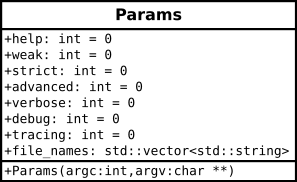
\includegraphics[width=0.4\linewidth]{obrazky-figures/class/params.pdf}
	\caption{Class diagram that shows inner representation of runtime arguments
	in Params class.}
	\label{fig:class:params}
\end{figure}

At the beginning is the \texttt{Params} class as we can see in Figure
\ref{fig:class:params}. In constructor of \texttt{Params} class is executed
getopt library to acquire a runtime arguments. The omitted arguments are then
saved in class variables. By this variables the whole tool is instrumented.

The next class diagram in Figure \ref{fig:class:ids} show us an Intermediate
Data Structure (IDS). The IDS is handled with multiple components in this
project, i.e., parser saves information there, etc., description is in Section
\ref{ids:description}. As you can see the \texttt{Argument} class has three
constructors.  Here could be used design pattern factory however, there are only
two different cases of creating an object so it was not needed. The
\texttt{Argument} class contains individual data about argument, e.g., the
format value says if the argument is in 'key=value' or 'value' form. The actual
value is stored in container \texttt{std::variant} that can contain two types,
\texttt{unsigned long} or \texttt{std::string}. This is the C++17 equivalent of
enumeration in C language.

\begin{figure}[H]
	\centering
	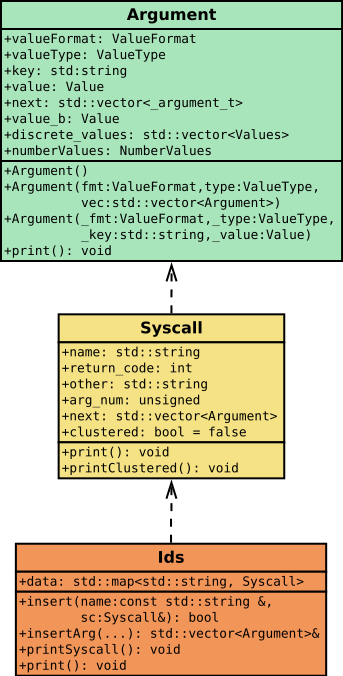
\includegraphics[width=0.45\textwidth]{obrazky-figures/class/arg_sc.pdf}
	\caption{Here we can see the intermediate data structure represented in
	class diagram. The whole IDS class contains list of syscalls, and syscalls
	contains arguments represented as a tree structure described in chapter
	earlier.}
	\label{fig:class:ids}
\end{figure}

\texttt{Syscall} class in Figure \ref{fig:class:ids} is dependant  on the
\texttt{Argument}. This class contains information about syscall, e.g.,
name, number of arguments, and actual arguments. There is defined
\texttt{print()} method that can print structurized data from syscall.

Class \texttt{Ids} in Figure \ref{fig:class:ids} describes the whole IDS. In
this class is located class variable of type \texttt{std::map<std::string,
Syscall>} wich hold syscall data. This means that \texttt{Ids} class is
dependant on class \texttt{Syscall}. The \texttt{Ids} class includes methods,
e.g., for structuralized print of whole class, or syscall only. It has
implemented method for inserting new Syscall object into the map.

The Figure \ref{fig:class:algo} illustrate dependency and generalization in class
hierarchy in the optimizer. As you can see the \texttt{Optimizer} is dependent
on \texttt{Algorithm} class. The \texttt{Algorithm} class is generalized by
specific algorithms, e.g., \texttt{Algo\_strict} class or
\texttt{Algo\_advanced} class. The optimizer contains a pointer to the
\texttt{Algorithm}. By this mechanism, it is really simple to change the
algorithm in the optimizer and keep the logical structure. It contains methods
for initializing and removing algorithm from an object. The algorithms have to
override the \texttt{optimize} method in \texttt{Algorithm} class thus it is
pure virtual in the base class. Because of that the compiler requests the
implementation of optimize method in a new class that inherits from
\texttt{Algorithm} class. The generalization is used for simple extension of
algorithms in the current solution. Every algorithm includes supportive methods
for the optimization, e.g., \texttt{Algo\_weak} has implemented method , e.g.,
\texttt{getMinMax}.

\begin{figure}[H]
	\centering
	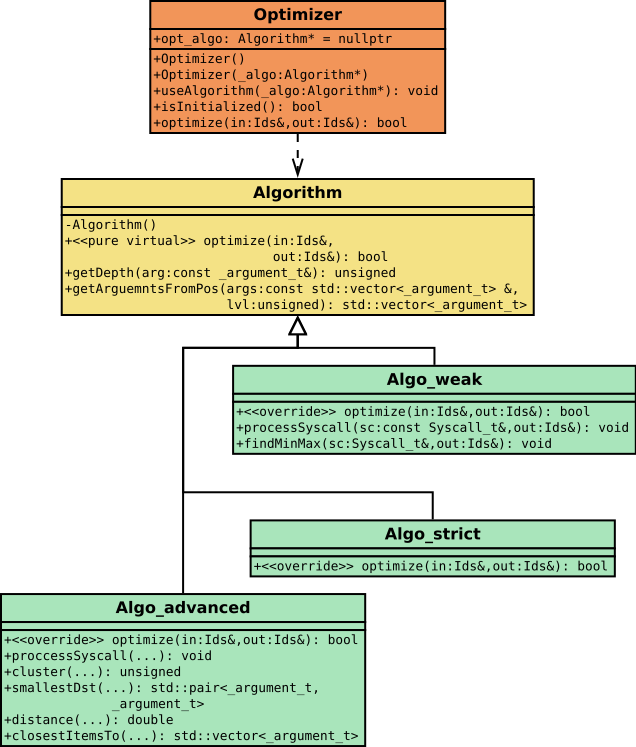
\includegraphics[width=0.8\textwidth]{obrazky-figures/class/algo.pdf}
	\caption{In this picture we can see a class diagram that describes
	a relationship among algorithms and optimizer. The optimizer contains pointer
	to the Algorithm class. The Algorithm class is used as an interface for
	the specific implementations. The implementations of algorithms, e.g, weak
	inherits the interface from Algorithm class and thus the optimizer can
	optimize with different algorithm implementations.}
	\label{fig:class:algo}
\end{figure}

In the Policy generator is used the same approach as in the optimizer. The
hierarchy among classes in policy generator shows the Figure
\ref{fig:class:output}. As we can see there is \texttt{Generator} class which is using
d-pointer pattern. \texttt{Generator} class contains a pointer to the \texttt{Output} class which
implements the specific output generator. This design supports a natural
expansion of generator implementations for other languages as well, e.g., Go or
Python.

In our case, we created support for C/C++ language and this support is
implemented in a class named \texttt{outputCPP}. This class contains multiple
methods, some of them are used for clustered IDS, and some of them are used for
unclustered IDS. Here are located filenames of a template for C/C++ function
wrapper of the generated filter. The output file can be changed with a
\texttt{setOutput} method. The printing into a file is implemented in batches.
It means that multiple rules for one syscall are printed at once.

\begin{figure}[H]
	\centering
	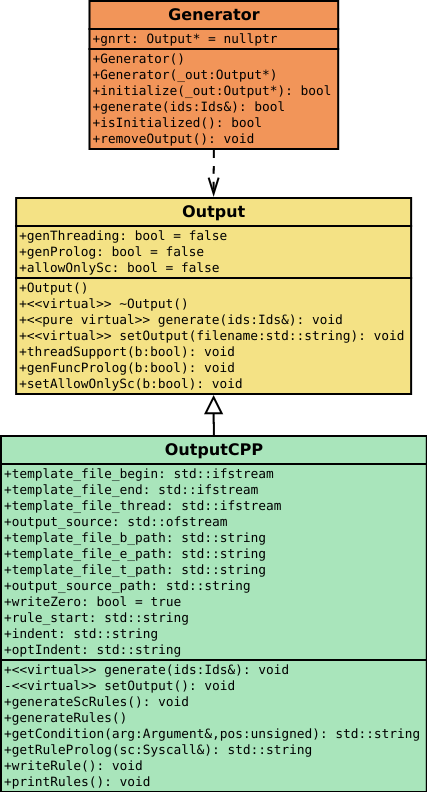
\includegraphics[width=0.45\linewidth]{obrazky-figures/class/output.pdf}
	\caption{In this Figure we can see relationship between generator and output
	implementation. Here is used the same approach as in the optimizer.
	The Generator contains pointer to the Output class which is interface for
	policy. In our case we implemented the policy generator for the C/C++.}
	\label{fig:class:output}
\end{figure}

\section{Used software}
In this section, I want to mention which software I used to develop a strace2seccomp tool.
Firstly, I mention compilers used in this project and after that valuable tools for developments.

\subsection{Compilers}
\label{subsec:compilers}
In this project, I used two compilers. The reason is simple.
Every compiler can detect a different set of errors and warnings during the compilation.
And at the time of doing project one of the reasons of compiling with two compilers
was to compare the execution times with optimizations turned on.

In the project, \texttt{libc++} and \texttt{libc++ ABI} from LLVM project was
used. The reason for using implementation from LLVM project was that in the GNU
implementation, there was a bug which affected a C++17
functionality\footnote{\url{https://bugs.debian.org/cgi-bin/bugreport.cgi?bug=877838}}
\footnote{\url{https://gcc.gnu.org/viewcvs/gcc?view=revision&revision=258854}}.
However, during the later development phase was the bug fixed and both implementation
of the library can be used.

\paragraph{GNU Compiler Collection.}GNU Compiler Collection is a part of the GNU project.
It aims to improve compiler used in the GNU ecosystem.
GCC\footnote{\url{https://gcc.gnu.org/}} uses an open development environment.
It includes front ends for C, C++, Objective-C, Go etc.
as well as libraries for these languages. It was firstly written for GNU operating system\footnote{\url{https://www.gnu.org/gnu/thegnuproject.html}}.
The compiler collection is released under the GPL license, other components, e.g., as runtime libraries are distributed under various free licenses.

\paragraph{LLVM/Clang.}
The goal of Clang\footnote{\url{https://clang.llvm.org/}} project is to provide a new C based language front-end (C, C++, Objective-C,) for the LLVM\footnote{\url{http://www.llvm.org/}} compiler.
It is released under NCSA Open Source license. Clang is designed to be highly compatible with GCC.
It supports most of the GCC compilation flags and unofficial language extensions\footnote{\url{https://clang.llvm.org/docs/LanguageExtensions.html}}.

\subsection{Dynamic and Static Code Analysis}
For correct development is necessary to find as many bugs as possible during this phase.
This goal was achieved by ussing dynamic and static analysis tools.
For static analysis was used an LLVM project named clang-tidy and for

\paragraph{LLVM/Clang-tidy.}
Clang-tidy is a clang-based ''linter'' tool\footnote{\url{http://clang.llvm.org/extra/clang-tidy/}}.
Its purpose is to diagnose and fix typical programming errors,
like interface misuse, style violation, or bugs that can be deduced via static analysis.
Clang-tidy diagnostics are designed to assert code that has invalid coding standard or is otherwise problematic.
It has options to disable some false positive warnings (e.g. \texttt{\textbackslash\textbackslash NOLINT}).

\paragraph{AddressSanitizer.}
AddressSanitizer\footnote{\url{https://github.com/google/sanitizers/wiki/AddressSanitizer}} (ASan) is a memory error detector for C/C++ developed by Google.
ASan is very fast and the average slowdown of the instrumented program is \textasciitilde 2x.
The tool consists of a runtime library which replaces the \texttt{malloc} function and compiler module (currently as LLVM pass).
The tool supports multiple architectures, e.g., x86, x86\_64, ARM, ARM\_64, MIPS, PowerPC64, etc.
It is part of the both compilers mentioned above in Subsection \ref{subsec:compilers}.

Usage of ASan is very straightforward. You have to only add compiler arguments:\\
\begin{center}
	\texttt{-fsanitize=address,undefined -fno-omit-frame-pointer}
\end{center}
The first parameter turns on the ASan and sanitizer for undefined behavior. The
second one prints a nicer stack trace in error messages. It is advised by
developers to use optimization, e.g., \texttt{-O1}, to get reasonable
performance.

\subsection{Miscellaneous}
This section describes miscellaneous software used in the project, e.g., Artistic Style, \ldots
\paragraph{Git}
Git\footnote{\url{https://git-scm.com/about}} is a source code manager (SCM). It stands out of the group of SCMs by its branching model.
Git allows and encourage you to have multiple local or remote branches that can be entirely independent.
This provides features like:
\begin{itemize}
	\item Context Switching
	\item Feature Based Workflow
	\item Role-based Codelines
	\item Disposable Experimentation
\end{itemize}
Other benefit of Git is that it does nearly all operations locally.
This gives the tool huge speed advantage.
Git was built to work with Linux kernel, that means it can effectively handle large repositories.
The st2se used repository hosting on GitHub.

\paragraph{Artistic Style}
Astyle\footnote{\url{http://astyle.sourceforge.net/}} is a source code formatter
and beautifuller. Works with C, C++ Objective-C, C\# and Java programming
languages. The motivation to use this tool is to have uniform code style. Some
of the editors by default insert spaces instead of tabs when pressing a key.
Other editors have the abillity to insert space before tab lines to visually
enhance the code (Emacs). The solution to this problem is to use Artistic Style
formatter. It can normalize the source code by rules defined in a configuration
file provided by a developer of the project.

\paragraph{LCOV and GCOV}
LCOV\footnote{\url{http://ltp.sourceforge.net/coverage/lcov.php}} is an extension to GCOV, a GNU tool which can determine what parts of a program was executed while running particular testcase.
It can provide information about how many times that part of program was executed.
LCOV implements to GCOV following additional functionality:
\begin{itemize}
	\item HTML based output with coverage rates indicated by specific color, i.e., green is 100\% and red is 0\% coverage.
	\item Support for large projects. It allows you to browse over overview pages that shows coverage data
	by providing: a directory view, a file view and a source code view.
\end{itemize}
LCOV was designed like Git to support Linux kernel, but works as well on standard user space applications.
This tool uses line coverage technique and it is the poorest coverage from the coverage types point of view.

\pagebreak
\section{Usage}

This section describes how to run the strace2seccomp tool, what runtime arguments
it has and how to turn on different optimization algorithms.

\begin{table}[h]
\centering
	\begin{tabular}{||l|l|p{6cm}||}
	\hline
	\multicolumn{3}{||l||}{\textbf{General options}}              \\ \hline\hline
	short format & long format         & description \\ \hline
	\texttt{-h}           & \texttt{----help}              & print this message \\
	\texttt{-v}           & \texttt{----verbose}           & turn on verbose mode \\
	\texttt{-d}           & \texttt{----debug}             & turn on debug mode \\
	\texttt{-t}           & \texttt{----tracing}           & turn on tracing mode \\
	\texttt{-A}           & \texttt{----analyze-grammar}   & analyze grammar \\
	\texttt{-o=FILE}      & \texttt{----output=FILE}       &  set output file \\ \hline
	\end{tabular}
	\caption{General options overview}
	\label{my-label}
\end{table}

\begin{table}[h]
\centering
	\begin{tabular}{||l|l|p{6cm}||}
	\hline
	\multicolumn{3}{||l||}{\textbf{Configuration options}}              \\ \hline\hline
	short format & long format         & description \\ \hline
	\texttt{-w}           & \texttt{----weak}         & use weak algotirthm \\
	\texttt{-s}           & \texttt{----strict}       & use strict algotirthm \\
	\texttt{-a}           & \texttt{----advanced}     & use advanced algotirthm \\
	                      & \texttt{----thread}       & generate function prolog \\
	                      & \texttt{----prolog}       & add filter synchronization among threads/processes \\ \hline
	\end{tabular}
	\caption{Configuration options overview}
	\label{my-label}
\end{table}


\paragraph{Examples} \hspace{0pt} \\

In Figure \ref{exec/run1}, we can see that verbose mode is turned on and minimax
algorithm was chosen for the optimizer. The output of the program will be stored
in source.cpp. Files filename1 and filename2 will be used as input.

\begin{figure}[H]
	\lstset{style=npl}
\begin{lstlisting}
> ./st2se -v -w --output=source.cpp filename1 filename2
\end{lstlisting}
	\caption{Running st2se with verbose mode, weak optimization, policy
	will be printed into \texttt{source.cpp} file, and input will read from
	\texttt{filename1} and \texttt{filename2}.}
	\label{exec/run1}
\end{figure}

The command in Figure \ref{exec/run2} diverges only in the output format and
used optimization algorithm. The \texttt{--thread} will generate support for
multithread or multiprocess applications and \texttt{--prolog} switch ensures
that the filter will be located in function. This behavior is helpful for copy \&
paste output into an existing program. The \texttt{-a} turns on the advanced
algorithm for IDS optimization.

\begin{figure}[H]
	\lstset{style=npl}
\begin{lstlisting}
> ./st2se -a --output=source.cpp filename --thread --prolog
\end{lstlisting}
	\caption{Running st2se with advanced optimization algorithm, output will be
	printed into a \texttt{source.cpp} file, \texttt{filename} will be used as
	input file, \texttt{----thread} switch will enable the synchronization of
	the policy 	among threads, \texttt{----prolog} switch will generate function
	wrapper for copy and paste policy into the code.}
	\label{exec/run2}
\end{figure}

When we want to check if the grammar in the parser is correct, we can use a
built-in tool in parser library. This tool of the parser can be turned on with
switch \texttt{-A}. Afterwards on standard output will be printed number of
found issues. This behavior we can see in Figure \ref{exec/run3}

\begin{figure}[H]
	\lstset{style=npl}
\begin{lstlisting}
> ./st2se -A
\end{lstlisting}
	\caption{Example of running st2se with option \texttt{-A} which turns on
	a grammar analysis. This functionality is provided from the parser library
	and is useful when we want to edit the parsing grammar and check for errors
	in it.}
	\label{exec/run3}
\end{figure}

\chapter{Software Verification}
This chapter will describe activities used to assure quality control of the
developed tool. First, I want to introduce on which aspects we will focus. One
of the aspects is \textit{module testing}. The main purpose of module testing is
to detect errors in submodules, in communication among them and in passing data
through data structures. Another aspect of verification is \textit{system
testing} merged with \textit{acceptance testing}. In this type of testing, we
will check if the strace2seccomp tool has a valid architectural design. Next, we
will check code with \textit{static analysis} tool and get information about
errors in code. Static analysis is type of testing which does not require to run
the program but requires a source code of the tool. The static analyzer will
analyze the source codes with different heuristics and produces a list of
detected errors.


\section{Module Testing}
Module testing is a part of the whole quality control process.
This testing can provide us how functional are particular components and if they meet the requirements.
Table \ref{table:moduletesting} shows us the description of module's test suits.

\begin{table}[h]
	\centering
	\begin{tabular}{||l|p{10cm}||}
		\hline
		\textbf{Module / Component}	&	\textbf{Test descriptiom} \\ \hline \hline
		Argparse					& Validity of recognized runtime arguments \\ \hline
		Generator					& Check methods functionality \\ \hline
		IDS							& Validity of constructors and class methods \\ \hline
		Output                      & Check the validity of generated policy \\ \hline
		States						& Check the getters and setter of states \\ \hline
		StraceParser				& Validity of all parser states by fuzzing \\ \hline
	\end{tabular}
	\caption{Test plan}
	\label{table:moduletesting}
\end{table}

For module testing was chosen Catch\footnote{\url{https://github.com/catchorg/Catch2}}
framework. This framework was chosen for its essential features which are:
\begin{itemize}
	\item one header library,
	\item no external dependencies,
	\item only one core assertion macro,
	\item tests can be tagged, and you can run only selected groups of tests,
	\item supports BDD\footnote{behavior Driven Development} and
	TDD\footnote{Test Driven Development} which can be used for next development
	cycle.
\end{itemize}

\paragraph{Params Testing}
Testing of the parameters was done manually which means by systematically
picking border values or some invalid ones and providing them as runtime
arguments for the strace2seccomp tool. It was automated with a handmade script.

\paragraph{Generator}
This test insists on setting class variables with class methods. The only reason
for this is that this class is used as abstract and thus we check only setters.

\paragraph{IDS}
This module test has multiple test cases. Here are tested constructors for
\texttt{Argument} structure, it has tree constructors. Next, there are tested
comparison operators for \texttt{Argument} class. After that, there is a test
for insertion into \texttt{Ids}. Another test case consists of support
functions of IDS module.

\paragraph{Output}
The output module test checks if the generated output is the same as expected
output. This test is considered as complicated because it depends on insertion
arguments into IDS, reading data from IDS and setting up the output generator.
This module test includes a test for setting class variables as well as the
module tests mentioned above.

\paragraph{States}
This module is crucial for the parser, so it is essential to have good module
test. In this test, we are checking the constructor, setters and getters and
class methods.

\paragraph{Module tests execution}
In Figure \ref{exec/unit_tests}, you can see how to run module tests from project
root directory.

\begin{figure}[h]
	\lstset{style=npl}
\begin{lstlisting}
> make check
\end{lstlisting}
	\caption{Example of running module tests from project root directory.}
	\label{exec/unit_tests}
\end{figure}

\paragraph{Results}
For module testing was implemented eleven test cases. In these test cases were
tested almost every class method and other functions in modules. Some test cases
were small, and they were testing only small methods and the others were more
complex and was designed to test the whole module. In conclusion, there were
eleven test cases with forty-two assertions, and all of them were satisfied.


\subsection{StraceParser Testing}
StraceParser module is responsible for parsing the strace output and translating
it into an intermediate data structure. Testing of this module can be done with
various techniques. First one which is used is fuzzy testing or fuzzing
described in the section below \ref{fuzzing}.

\subsubsection{Fuzzing}
\label{fuzzing}
The term fuzzing was first used by professor Barton Miller who used fuzzing to
test robustness of UNIX applications in 1989 \cite{Takanen:2008:FSS:1404500,
Marhefka2013}. Fuzzing is a testing method which generates an unexpected input
on tested software and then is observing if the software crashes. The whole
process is typically automated or semiautomated which involves repeatedly
manipulating and supplying input data to the targeted program. Some modern
fuzzers (programs that generates a stochastic input) record every crash or halt
of a tested program. The stochastic data are in the most cases invalid to
observer thus he can see how application handles invalid states and boundary
conditions. The name comes from modern applications tendency to fail due to
random input caused by line noise on \emph{fuzzy} telephone lines
\cite{Takanen:2008:FSS:1404500, N2LYDLnqzEFYp0wM, takanen2009fuzzing}. In other
literature, fuzzing can be named by these terms:
\begin{itemize}
	\item Negative testing
	\item Syntax testing
	\item Dirty testing
	\item Robustness testing
	\item Protocol mutation
	\item Fault injection
\end{itemize}

\noindent
Fuzzers can be divided into two large groups:

\begin{itemize}
	\item \textbf{Generation-based} fuzzers creates test suite from scratch by modeling the target grammar.
	\item \textbf{Mutation-based} fuzzers needs an (in)valid input file. The file is mutated by various techniques.
	The mutation can be e.g. bitflip, byte change, duplicate or swap some chunks in the input file.
	The mutated test case is then provided to a tested program.
\end{itemize}

For us \emph{Mutation-based} group is interesting because it is easier to setup and
is more available in open source community. There are many options to choose so here is
a little comparison of most popular fuzzers:

\begin{itemize}

	\item \textbf{Bunny the Fuzzer}\footnote{\url{https://code.google.com/archive/p/bunny-the-fuzzer/}} is a closed loop, general purpose fuzzer for C programs.
	The fuzzer uses compiler-level integration which means that it injects reliable instrumentation hooks into an object file.
	Those hooks enable the fuzzer to trace the program, and can provide real-time feedback. This architecture provides a possibility
	to considerably improve coverage of testing process. The injection of the hooks
	needs to be done by the compiler scripts.
	This fuzzer subset of American Fuzzy Lop. This project is now deprecated.

	\item \textbf{American Fuzzy Lop}\footnote{\url{http://lcamtuf.coredump.cx/afl/}}
	is a security oriented fuzzer that add compile-time instrumentation. It is
	supperset to really similar Bunny the Fuzzer. The fuzzer has implemented many
	researched fuzzing capabilities (bit / byte flips,  simple arithmetics, known
	integers, test case splicing, \ldots). Compared to other instrumented fuzzers it
	has moderate overhead and as little configuration as possible. The disadvantage
	of the tool is that it needs to be executed multiple times to achieve
	multiprocess or multithread fuzzing.

	\item \textbf{Honggfuzz}\footnote{\url{http://honggfuzz.com/}} is an evolutionary, security oriented, easy to use fuzzer with analysis options.
	The main advantage of this mutation based fuzzer is that it is multi-process and multi-threded without need to run multiple copies of fuzzer.
	The file corpus is automatically shared and improved among the processes / threads.
	Authors of the fuzzer says that it is blazing fast when it works in persistent fuzzing mode'.
	For monitoring of target (process under test) it uses {\textcolor{red}{a}} low-level interface (e.g ptrace in Linux).
	It supports several hardware based (Intel BTS, Intel PT) and software based fuzzing methods.

	\item \textbf{Radamsa} is fuzzing tool\footnote{\url{https://github.com/aoh/radamsa}} developed at the Oulu university.
	The motivation for building this fuzzer was to make robustness testing accessible to independent developers.
	The existing tools were considered hard to use and to customize to fit the project.
	The fuzzer is a command line tool, on input it expects multiple files (samples), and generates mutated files.
	So, by the output Radamsa is considered as a mutation-based fuzzer.
	The tool includes feature aiding in automatizing test runs.
	This is achieved by specifying number of wanted test runs with unique mutated files.
	Another parameter that can be set is a random seed for mutation.
	On the other hand, the tool does not provide an option to monitor target (program under test).
	Radamsa is a multiplatform so it is built for Windows and Linux \cite{radamsaThesis}.

	\item \textbf{Oss-fuzz} is a complex project developed by Google\footnote{\url{https://github.com/google/oss-fuzz}}.
	The architecture of this project is that the ClusterFuzz (fuzzer tools)
	automatically pulls the newest source code from repository and it will starts
	fuzzers and sanitizers \footnote{Dynamic testing tool that can detect bugs and
	faults during the execution. Typical sanitizers are \textit{ASan},
	\textit{DFSan}, \ldots}. When some bug or fault occurs, it is automatically
	reported to the OSS-fuzz issue tracker. Project owners are then notified with
	an email about the issue. When the fix is submitted ClusterFuzz automatically
	verifies the fix, adds a comment to issue tracker and closes the issue.

\end{itemize}


\subsubsection{Fuzzing results}
The chosen fuzzer was AFL for its ability of fast deployment and easy of use.
The opposite example is Oss-fuzz which is the whole infrastructure for fuzzing and bug hunting.

In fuzzed program, only parsing was enabled every other module was turned off.
The fuzzer run straight twenty-one days and during this time it was discovered
three false positive hangs and no crashes. Fuzzing runs in four threads on Intel
Core i7-4810MQ. Overall the fuzzed program was executed 3,567,228,619 times.

The number of executions per second was not stable on master thread because it
was necessary to instrument other three processes. This instability can be
seen among Figures \ref{fuz:result1a}, \ref{fuz:result2a}, \ref{fuz:result3a}
and \ref{fuz:result4a}.

\begin{figure}[H]
	\centering
	\includegraphics[width=0.8\linewidth]{obrazky-figures/master/exec_speed.pdf}
	\caption{Execution speed on thread no.1. As we can see, the execution speed
	is not constant, but it oscilates due to instrumentation of other threads. }
	\label{fuz:result1a}
\end{figure}

\begin{figure}[H]
	\centering
	\includegraphics[width=0.8\linewidth]{obrazky-figures/thread_1/exec_speed.pdf}
	\caption{Execution speed on thread no.2. We can see that the execution speed
	is constant.}
	\label{fuz:result2a}
\end{figure}

\begin{figure}[H]
	\centering
	\includegraphics[width=0.8\linewidth]{obrazky-figures/thread_2/exec_speed.pdf}
	\caption{Execution speed on thread no.3. We can see that the execution speed
	is constant.}
	\label{fuz:result3a}
\end{figure}

\begin{figure}[H]
	\centering
	\includegraphics[width=0.8\linewidth]{obrazky-figures/thread_3/exec_speed.pdf}
	\caption{Execution speed on thread no.4. We can see that the execution speed
	is constant.}
	\label{fuz:result4a}
\end{figure}
%
% asdfasdfasf
% asdfasdfasf
% asdfasdfasf
%
% \begin{figure}[H]
% 	\centering
% 	\includegraphics[width=\linewidth]{obrazky-figures/master/high_freq.pdf}
% 	\caption{master/high\_freq}
% 	\label{fuz:result1b}
% \end{figure}
%
% \begin{figure}[H]
% 	\centering
% 	\includegraphics[width=\linewidth]{obrazky-figures/thread_1/high_freq.pdf}
% 	\caption{thread\_1/high\_freq}
% 	\label{fuz:result2b}
% \end{figure}
%
% \begin{figure}[H]
% 	\centering
% 	\includegraphics[width=\linewidth]{obrazky-figures/thread_2/high_freq.pdf}
% 	\caption{thread\_2/high\_freq}
% 	\label{fuz:result3b}
% \end{figure}
%
% \begin{figure}[H]
% 	\centering
% 	\includegraphics[width=\linewidth]{obrazky-figures/thread_3/high_freq.pdf}
% 	\caption{thread\_3/high\_freq}
% 	\label{fuz:result4b}
% \end{figure}
%
% asdfasdfasfasdfasdfasfasdfasdfasfasdfasdfasf
%
% \begin{figure}[H]
% 	\centering
% 	\includegraphics[width=\linewidth]{obrazky-figures/master/low_freq.pdf}
% 	\caption{master/low\_freq}
% 	\label{fuz:result1c}
% \end{figure}
%
% \begin{figure}[H]
% 	\centering
% 	\includegraphics[width=\linewidth]{obrazky-figures/thread_1/low_freq.pdf}
% 	\caption{thread\_1/low\_freq}
% 	\label{fuz:result2c}
% \end{figure}
%
% \begin{figure}[H]
% 	\centering
% 	\includegraphics[width=\linewidth]{obrazky-figures/thread_2/low_freq.pdf}
% 	\caption{thread\_2/low\_freq}
% 	\label{fuz:result3c}
% \end{figure}
%
% \begin{figure}[H]
% 	\centering
% 	\includegraphics[width=\linewidth]{obrazky-figures/thread_3/low_freq.pdf}
% 	\caption{thread\_3/low\_freq}
% 	\label{fuz:result4c}
% \end{figure}
%
% asdfasdfasfasdfasdfasfasdfasdfasfasdfasdfasfasdfasdfasf

% \subsection{Algorithms}
% How should we test the algorithms?

\section{System and Acceptance Testing}
\label{acceptance_testing}
In the book of Software Acceptance Testing, acceptance testing is defined as:
''Acceptance testing is the formal testing activity that presents the
product to the customer by enterprise (many times it includes stakeholders as
well). This activity represents demonstration of a software product and shows to
the customer that the requirements fulfilled its obligations. By this activity
you can decide if the product is ready for deployment. The software items must
be examined to ensure that the provided product is complete, i.e., the
architecture must be audited to check if it accurate reflects the software
configuration. The test results are audited by functional configuration audit to
certify that the software product satisfies its specification etc.''
\cite{Schmidt2013335}.

Acceptance testing will consist of steps as generate policies, i.e., a whitelist
of system calls from strace of given program and applying the whitelist into
carefully picked programs. Afterwards, we run the testsuite provided for that
program and by this way we can immediately see if the generated whitelist works
correctly.

\subsection{Testing on real programs}
For this testing four programs was picked. RedHat Inc. demands one, and that is
USBGuard\footnote{\url{https://usbguard.github.io/}}. USBGuard is an open source
project developed under GNU GPL v2.0 license. It implements USB device
authorization which can be set up locally or with centralized
management \cite{usbguardCentralized}. USBGuard has a sophisticated architecture
which is complicated enough for use in this testing. Another advantage of
USBGuard is that it has large enough testsuite which will be helpful in the
evaluation of generated policies by \texttt{strace2seccomp}. In this project, we
will focus only on a daemon because it is most involved in the whole project.

Next program is called \emph{cp} which is part of a GNU project called
\emph{coreutils}\footnote{\url{https://www.gnu.org/software/coreutils/coreutils.html}}.
The \emph{cp} is a program used for copying files across filesystem typically on
POSIX operating systems. One of the advantages of this project is that it has a
relatively big testsuite. The drawback of this program is that it is a part of a
big project and is tough to acquire strace logs from testsuite. This problem I
solved by manually patching the Makefile which was responsible for running
tests. The patch will add strace command with appropriate flags before the
invocation of \emph{cp}.

Another program is \emph{find} from GNU project called
\emph{findutils}\footnote{\url{https://www.gnu.org/software/findutils/}}. The
\emph{find} is a program used to locate files or directories in filesystem. It
is specific for GNU Linux as well as cp. This program has good testsuite as a
\emph{coreutils} project does. The drawback of the project complexity is similar to
\emph{coreutils}. In \emph{find} is a high number of system calls that differ
only in provided arguments thus it will test the robustness of clustering in the
\texttt{strace2seccomp} tool.

The last program is a school project from \emph{Network Applications} class called
\emph{testovac}\footnote{\url{https://github.com/tammar96/ISA-testovac}}. This
project was chosen for its multithreaded architecture. With this program, we can
test if the filter is successfully distributed on other threads. The
\emph{testovac} does not have a good testsuite thus we only run it in one
scenario. However, the point of this test is to see if the provided seccomp
filter works on multithreaded applications.

\subsection{Test Preparation}
For the testing, we need to set up an environment. For this purpose, we have
a~script which will download software on which will be stare2seccomp tested. The
script is named \texttt{./setEnv} and is located in testsuite folder.
The script has multiple subcommands:
\begin{itemize}
	\item \texttt{prep} will download, extract and configure tested programs
		(\emph{coreutils}, \emph{findutils}, USBGuard, \emph{testovac})
	\item \texttt{applyPolicy} will patch source codes with generated policies
	\item \texttt{make} will run make for all tested programs
	\item \texttt{tests} will run testsuits
	\item \texttt{clean} will clean the testing folder
	\item \texttt{revertPatches} will revertPatches
	\item \texttt{straceON} will turn on strace output while running testsuite
	\item \texttt{straceOFF} will turn off strace output while running testsuite
\end{itemize}

\begin{figure}[H]
  \centering
  \resizebox {0.8\textwidth} {!} {
    \begin{tikzpicture}
	\begin{pgfonlayer}{nodelayer}
		\node [] (0) at (-9, 4) {};
		\node [] (1) at (-9, 3) {};
		\node [] (2) at (-7, 3) {};
		\node [] (3) at (-7, 4) {};
		\node [] (4) at (-7, 3.5) {};
		\node [] (5) at (-6, 3.5) {};
		\node [] (6) at (-6, 4) {};
		\node [] (7) at (-6, 3) {};
		\node [] (8) at (-4, 3) {};
		\node [] (9) at (-4, 4) {};
		\node [] (10) at (-4, 3.5) {};
		\node [] (11) at (-3, 3.5) {};
		\node [] (12) at (-3, 4) {};
		\node [] (13) at (-3, 3) {};
		\node [] (14) at (-1, 4) {};
		\node [] (15) at (-1, 3) {};
		\node [] (16) at (-1, 3.5) {};
		\node [] (17) at (0, 3.5) {};
		\node [] (18) at (0, 4) {};
		\node [] (19) at (0, 3) {};
		\node [] (20) at (1, 3) {};
		\node [] (21) at (2, 4) {};
		\node [] (22) at (2, 3) {};
		\node [] (23) at (-8, 3.5) {prep};
		\node [] (24) at (-5, 3.5) {straceON};
		\node [] (25) at (-2, 3.5) {make};
		\node [] (26) at (1, 3.5) {tests};
		\node [] (27) at (1, 2) {};
		\node [] (28) at (0, 2) {};
		\node [] (29) at (0, 1) {};
		\node [] (30) at (2, 1) {};
		\node [] (31) at (2, 2) {};
		\node [] (32) at (0, 1.5) {};
		\node [] (33) at (-0.75, 1) {};
		\node [] (34) at (-0.75, 2) {};
		\node [] (35) at (-3.25, 2) {};
		\node [] (36) at (-3.25, 1) {};
		\node [] (37) at (-4, 1) {};
		\node [] (38) at (-4, 2) {};
		\node [] (39) at (-6, 2) {};
		\node [] (40) at (-6, 1) {};
		\node [] (41) at (-7, 1) {};
		\node [] (42) at (-7, 2) {};
		\node [] (43) at (-9, 2) {};
		\node [] (44) at (-9, 1) {};
		\node [] (45) at (-0.75, 1.5) {};
		\node [] (46) at (-3.25, 1.5) {};
		\node [] (47) at (-4, 1.5) {};
		\node [] (48) at (-6, 1.5) {};
		\node [] (49) at (-7, 1.5) {};
		\node [] (50) at (-9, 1.5) {};
		\node [] (51) at (1, 1.5) {straceOFF};
		\node [] (52) at (-2, 1.5) {applyPolicy};
		\node [] (53) at (-5, 1.5) {make};
		\node [] (54) at (-8, 1.5) {tests};
	\end{pgfonlayer}
	\begin{pgfonlayer}{edgelayer}
		\draw (0.center) to (3.center);
		\draw (3.center) to (4.center);
		\draw (4.center) to (2.center);
		\draw (2.center) to (1.center);
		\draw (1.center) to (0.center);
		\draw [decoration={markings,mark=at position 1 with {\arrow[scale=2]{>}}},
    postaction={decorate}] (4.center) to (5.center);
		\draw (5.center) to (6.center);
		\draw (6.center) to (9.center);
		\draw (9.center) to (10.center);
		\draw (10.center) to (8.center);
		\draw (8.center) to (7.center);
		\draw (7.center) to (5.center);
		\draw [decoration={markings,mark=at position 1 with {\arrow[scale=2]{>}}},
    postaction={decorate}] (10.center) to (11.center);
		\draw (11.center) to (12.center);
		\draw (13.center) to (11.center);
		\draw (13.center) to (15.center);
		\draw (14.center) to (12.center);
		\draw (14.center) to (16.center);
		\draw (16.center) to (15.center);
		\draw [decoration={markings,mark=at position 1 with {\arrow[scale=2]{>}}},
    postaction={decorate}] (16.center) to (17.center);
		\draw (17.center) to (18.center);
		\draw (18.center) to (21.center);
		\draw (21.center) to (22.center);
		\draw (22.center) to (20.center);
		\draw (20.center) to (19.center);
		\draw (19.center) to (17.center);
		\draw (28.center) to (32.center);
		\draw (32.center) to (29.center);
		\draw (29.center) to (30.center);
		\draw (30.center) to (31.center);
		\draw (31.center) to (27.center);
		\draw (27.center) to (28.center);
		\draw [decoration={markings,mark=at position 1 with {\arrow[scale=2]{>}}},
    postaction={decorate}] (20.center) to (27.center);
		\draw (43.center) to (42.center);
		\draw (44.center) to (41.center);
		\draw (37.center) to (40.center);
		\draw (39.center) to (38.center);
		\draw (35.center) to (34.center);
		\draw (33.center) to (36.center);
		\draw (43.center) to (50.center);
		\draw (50.center) to (44.center);
		\draw (41.center) to (49.center);
		\draw (49.center) to (42.center);
		\draw (39.center) to (48.center);
		\draw (48.center) to (40.center);
		\draw (38.center) to (47.center);
		\draw (47.center) to (37.center);
		\draw (35.center) to (46.center);
		\draw (46.center) to (36.center);
		\draw (34.center) to (45.center);
		\draw (45.center) to (33.center);
		\draw [decoration={markings,mark=at position 1 with {\arrow[scale=2]{>}}},
    postaction={decorate}] (32.center) to (45.center);
		\draw [decoration={markings,mark=at position 1 with {\arrow[scale=2]{>}}},
    postaction={decorate}] (46.center) to (47.center);
		\draw [decoration={markings,mark=at position 1 with {\arrow[scale=2]{>}}},
    postaction={decorate}] (48.center) to (49.center);
	\end{pgfonlayer}
\end{tikzpicture}

  }
  \caption{Steps to set environment, gather strace logs, make binaries, run tests}
  \label{fig:tikz:setenv_architecture}
\end{figure}

\subsection{Test Requirements}
Requirements for the testing are:
\begin{enumerate}
	\item Internet connection - used for download tested software (findutils,
	coreutils, usbguard).
	\item Computer with x86 architecture - For testing purpose was chosen
	machine with x86 architecture.
\end{enumerate}

\subsection{Results}
During testing phase, multiple issues was discovered. The first issue is caused
by the libseccomp library which is not supporting intervals (ranges) in any way.
The libseccomp architecture specifies that in one function
\texttt{seccomp\_rule\_add} is logical and among partial expressions. Among the
functions \texttt{seccomp\_rule\_add} is logical or. Moreover, in one function
\texttt{seccomp\_rule\_add} argument position can be mentioned only once which
means that it is not possible to write intervals as shown in Figure
\ref{libseccomp_native}.

\begin{figure}[h]
	\label{libseccomp_native}
	\lstset{style=c++}
	\begin{lstlisting}
seccomp_rule_add(
	ctx,
	SCMP_ACT_ALLOW,
	SCMP_SYS(write),
	2,
	SCMP_A0(SCMP_CMP_GE, 1), SCMP_A0(SCMP_CMP_LE, 5) // interval
);
	\end{lstlisting}
	\caption{Possible range expression}
\end{figure}

This issue was partially solved in this pull
request\footnote{\url{https://github.com/seccomp/libseccomp/issues/94}}. The
problem with this pull request is that it is not confirmed if it will be merged
into libseccomp. Because of that, in this thesis a downstream version of
libseccomp which has to be manually installed on the system is used. In the downstream
version, interval can be expressed as shown in Figure \ref{libseccomp_in_range}.

\begin{figure}[h]
	\label{libseccomp_in_range}
	\lstset{style=c++}
	\begin{lstlisting}
seccomp_rule_add(
	ctx,
	SCMP_ACT_ALLOW,
	SCMP_SYS(write),
	1,
	SCMP_A0(SCMP_CMP_IN_RANGE, 1, 5) // interval
);
	\end{lstlisting}
	\caption{Proposed operator \texttt{SCMP\_CMP\_IN\_RANGE}}
\end{figure}

Another issue is that the libseccomp operators as
\texttt{SCMP\_CMP\_GT/GE/LT/LE} are not designed to work with negative values
provided to system calls. This issue is as well reported to the libseccomp
project\footnote{\url{https://github.com/seccomp/libseccomp/issues/69}}. Luckily
this problem is not as critical as the previously stated one. In the end the
the kernel is passing the arguments as unsigned and the interpretation of these values
is on the implementation of system call.

This situation we can see in particular cases. Very often it is a \texttt{mmap}
or \texttt{llseek}. The problem is nicely visible on the x86\_64 / amd64 architecture. The system call
numbers are 64bits wide numbers, and BPF used in the kernel uses only 32bits
wide registers. Libseccomp is generating a comparison of 64-bit number as a two
32-bits unsigned numbers. We can prove this with libseccomp code or by
disassembling BPF instructions generated by libseccomp.

Imagine that we have a clear filter so every system call would be killed. We add
only one rule which is shown in Figure \ref{libseccomp_rule}. This rule means
that fifth argument must be in the range $[-2, 3]$ including border values.

\begin{figure}[h]
	\label{libseccomp_rule}
	\lstset{style=c++}
	\begin{lstlisting}
ret |= seccomp_rule_add(ctx, SCMP_ACT_ALLOW, SCMP_SYS(mmap), 1,
	SCMP_A4(SCMP_CMP_IN_RANGE, -2, 3)
);
	\end{lstlisting}
	\caption{Only rule we are adding into a libseccomp filter}
\end{figure}

In Figure \ref{BPF_rule}, we can see the generated BPF code. The interesting part
begins on~line~5. Here we can see that the rule  which we specified in
C/C++ code begins. On~line~6, we store upper 32 bits of a number in accumulator.
On~line~7 begins we are comparing accumulator with value \texttt{0xffffffff} and then
on~line~8 with zero. This behavior is invalid and should be mentioned in documentation.

\begin{figure}[h]
	\label{BPF_rule}
	\lstset{style=npl}
	\begin{lstlisting}
line | CODE | JT | JF | K
=================================
0000: 0x20 0x00 0x00 0x00000004  A = arch
0001: 0x15 0x00 0x0b 0xc000003e  if (A != ARCH_X86_64) goto 0013
0002: 0x20 0x00 0x00 0x00000000  A = sys_number
0003: 0x35 0x00 0x01 0x40000000  if (A < 0x40000000) goto 0005
0004: 0x15 0x00 0x08 0xffffffff  if (A != 0xffffffff) goto 0013
0005: 0x15 0x00 0x07 0x00000009  if (A != mmap) goto 0013
0006: 0x20 0x00 0x00 0x00000034  A = args[4] >> 32 <--- storing upper 32bits
0007: 0x35 0x00 0x05 0xffffffff  if (A < 0xffffffff) goto 0013
0008: 0x25 0x04 0x00 0x00000000  if (A > 0x0) goto 0013
0009: 0x20 0x00 0x00 0x00000030  A = args[4] <--------- storing lower 32bits
0010: 0x35 0x00 0x02 0xfffffffe  if (A < 0xfffffffe) goto 0013
0011: 0x25 0x01 0x00 0x00000003  if (A > 0x3) goto 0013
0012: 0x06 0x00 0x00 0x7fff0000  return ALLOW
0013: 0x06 0x00 0x00 0x00000000  return KILL
	\end{lstlisting}
	\caption{Disassembled BPF filter on amd64 machine}
\end{figure}

As development continued, we discovered another issue that prevents from correct
functionality. This issue is occurring when we try to load seccomp filter in a
multithread application, and we want to synchronize it across threads or
processes. Already stated issue is mentioned in libseccomp issue
tracker\footnote{\url{https://github.com/seccomp/libseccomp/issues/93}} and
there is a working solution to this issue. However, there were many conflicts in
code when applying those patches, and even if we applied those patches, it was
in conflict with a previously applied patch that was the workaround for ranges.
Thus we decided to stick with range patch (it is more important than thread
support), and not with the multithread patches. In the end, there is still
implemented the multithread support in the developed tool without regard to
functionality in libseccomp. As we cannotice, one of the involved programs for
complex testing, testovac, cannot be tested.

In the testing phase was discovered issues in the generated filter as well. We
processed the strace logs for the \texttt{cp} command from coreutils projects
and manually checked with strace logs, and it was correctly created. The
troubles occurred when we tried to run the \texttt{cp}. Immediately after start,
it was terminated with signal \texttt{SIGSYS} and error message 'bad system
call' was emitted. We decided to troubleshoot where the problem occurs. When we
run strace on \texttt{cp} without runtime arguments, it shows us in Figure
\ref{cp_strace_error} that it was terminated when demanding system call
\texttt{openat}.
\begin{figure}[h]
	\label{cp_strace_error}
	\lstset{style=npl}
	\begin{lstlisting}
prctl(PR_SET_NO_NEW_PRIVS, 1, 0, 0, 0)  = 0
seccomp(SECCOMP_SET_MODE_STRICT, 1, NULL) = -1 EINVAL (Invalid argument)
seccomp(SECCOMP_SET_MODE_FILTER, 0, {len=281, filter=0x22fdaf0}) = 0
openat(AT_FDCWD, "/usr/lib/locale/locale-archive", O_RDONLY|O_CLOEXEC) = ?
+++ killed by SIGSYS (core dumped) +++
[1]    1941 invalid system call (core dumped)  strace ./cp
	\end{lstlisting}
	\caption{Part of the strace log of cp command}
\end{figure}

The \texttt{openat} has three arguments which are constant, path, and bitfield.
The path is not processed by our tool, so we will aim for the other two
arguments. The first one is \texttt{AT\_FDCWD} and it is defined in source file
\texttt{'/include/uapi/linux/fcntl.h'} with value '-100'. The bitfield
is located in file \texttt{'/include/uapi/asm-generic/fcntl.h'} and the macro
\texttt{O\_RDONLY} has value '0', and the \texttt{O\_CLOEXEC} macro has value
'02000000'. We dumped the bpf filter with libseccomp API and examined it. We
tried to emulate the system call with the seccomp-tools project as shown in
Figure \ref{emulation_cp}.

\begin{figure}[h]
	\lstset{style=npl}
\begin{lstlisting}
> seccomp-tools emu --arch amd64 ./seccomp_filter.bpf 257 18446744073709551516 0 02000000
\end{lstlisting}
	\caption{Seccomp-tools emulation of the \texttt{openat} syscall}
	\label{emulation_cp}
\end{figure}

We will break down that command. The \texttt{emu --arch amd64}  arguments say
that it will emulate an amd64 architecture, and after that is exported bpf
filter. The four last numbers are syscall number and its arguments.
The \texttt{openat} syscall has value 257, and the long number afterward is -100
transformed in 64-bit unsigned number. The second argument is zero but can be
any number because in the second position is the path and that is not processed
in our filter, and the last one is our bitfield. When we run the emulation tool,
and afterward we get the opposite result as we expected. The result is that the
system call will be allowed, but that does not correspond with binary. Next, we
should check the generated filter we put in the source code, shown in Figure
\ref{cp_seccomp_rule}.

\begin{figure}[h]
	\lstset{style=c++}
\begin{lstlisting}
ret |= seccomp_rule_add(ctx, SCMP_ACT_ALLOW, SCMP_SYS(openat), 2,
    SCMP_A0(SCMP_CMP_EQ, AT_FDCWD),
    SCMP_A2(SCMP_CMP_MASKED_EQ, O_RDONLY|O_CLOEXEC)
);
\end{lstlisting}
	\caption{Rule in generated filter by \texttt{strace2seccomp}}
	\label{cp_seccomp_rule}
\end{figure}


We can see that the filter has the rule for allowance that system call with that
combination of arguments. When we edit that rule manually as shown in Figure
\ref{cp_strace_error_2}, we can see that after running the cp command that it is
stoped at another syscall. That system call is \texttt{mmap}. In generated
filter (Figure \ref{cp_seccomp_rule_edit_1}) we can find that \texttt{mmap} is
not allowed with that value. However, the value was not present in the strace
logs, and when we change it, then our program is behaving correctly. We can
continue this way to the point where we remove all issues with the generated
filter. Those issues are not a product of the incorrect handling in
\texttt{strace2seccomp} tool, but they are the product of the small testsuite
provided by the project coreutils. The only thing that can be discussed is a
problem when handling file descriptors. Sometimes the program opens the same
file on a different file descriptor; thus it should not be processed.

\begin{figure}[h]
	\lstset{style=npl}
\begin{lstlisting}
prctl(PR_SET_NO_NEW_PRIVS, 1, 0, 0, 0)  = 0
seccomp(SECCOMP_SET_MODE_STRICT, 1, NULL) = -1 EINVAL (Invalid argument)
seccomp(SECCOMP_SET_MODE_FILTER, 0, {len=236, filter=0x23af210}) = 0
openat(AT_FDCWD, "/usr/lib/locale/locale-archive", O_RDONLY|O_CLOEXEC) = 3
fstat(3, {st_mode=S_IFREG|0644, st_size=209526528, ...}) = 0
mmap(NULL, 209526528, PROT_READ, MAP_PRIVATE, 3, 0) = ?
+++ killed by SIGSYS (core dumped) +++
\end{lstlisting}
	\caption{Part of the strace log of cp command}
	\label{cp_strace_error_2}
\end{figure}

\begin{figure}[h]
	\lstset{style=c++}
\begin{lstlisting}
ret |= seccomp_rule_add(ctx, SCMP_ACT_ALLOW, SCMP_SYS(mmap), 1,
    SCMP_A1(SCMP_CMP_IN_RANGE, 16u, 3926752u)
);
\end{lstlisting}
	\caption{Rule in generated filter by \texttt{strace2seccomp}}
	\label{cp_seccomp_rule_edit_1}
\end{figure}

This analysis points to the conclusion that there is a reason to check the
advanced algorithm DBSCAN because seccomp incorrectly interpreted even the
minimax algorithm generated by strace2seccomp tool. There is no point even in
testing the find tool because there would be the same problem.

\chapter{Conclusion}
Nowadays, if we want to block malicious software we can use some software that
will terminate the process based on its behavior in system or we can use
in-compiled policy that will terminate the program when it starts calling system
call which was not allowed. This is done by seccomp by manually creating such
policies.

Within this thesis, We succesfully designed and implemented a tool that can
translate a strace log into the libseccomp policy. To achieve the translation, we
had to solve multiple problems. First of them was to create a simple inner data
structure which will represent the whole strace log without duplicit
information. The other problem we faced was to parse the strace log. In our
case, we used PEGTL library which was not the fastest solution, but it was simple
to prototype grammar with it. Another issue was to optimize and simplify the
data structure. We implemented three algorithms (strict, weak, advanced). The
implementation was designed with design patterns to be easily extended with new
optimization algorithms. The last problem of development phase was to create
policy generator. We implemented the same design pattern as in the optimizer, to
provide extensibility of policy generator for other languages. We decided to
implement the policy generator that creates policy in C/C++.

The most interesting part of this thesis is the testing phase. During this phase
we discovered multiple issues that prevent from correct policy interpretation.
One of them is that the libseccomp library does not provide \emph{in range}
operator yet. This operator prevents the correct policy generation for weak
algorithm. The other discovered problem was the interpretation of the policy by
seccomp. The seccomp terminated system call even if the policy contained the
rule that allows the syscall. These issues were preventing us from
complex testing of the developed tool.

This thesis can be extended with another optimization algorithms or different
implementations of policy generator, i.e, add support for other languages (Go).
These extensions can be done as another dedicated thesis.


%=========================================================================
